\documentclass[10pt,letterpaper]{article}

\usepackage[utf8]{inputenc}
\usepackage[T1]{fontenc}
\usepackage{amsmath,amssymb,amsthm,mathtools}
\usepackage{array,booktabs,longtable,multirow,tabularx}
\usepackage{authblk}
\usepackage{caption}
\usepackage{enumitem}
\usepackage{float}
\usepackage{geometry}
\usepackage{graphicx}
\usepackage{microtype}
\usepackage[numbers,sort&compress]{natbib}
\usepackage[most]{tcolorbox}
\usepackage{xcolor}
\usepackage{url}
\usepackage{xurl}
\usepackage[colorlinks=true,bookmarksopen=true,bookmarksnumbered=true,
  citecolor=red!70!black,linkcolor=blue!55!black,urlcolor=red!65!black,
  pdfauthor={Dhruv Sharma},
  pdftitle={CHMT-Q: Causal Hierarchical Market Transformer with Quantiles}]{hyperref}

\geometry{left=2cm,right=2cm,top=1cm,bottom=1.25cm}
\setcounter{secnumdepth}{3}
\setcounter{tocdepth}{2}
\numberwithin{equation}{section}
\setlist{nosep,leftmargin=1.5em}
\captionsetup{font=small,labelfont=bf}
\renewcommand{\arraystretch}{1.12}
\newcommand{\E}{\mathbb{E}}
\newcommand{\R}{\mathbb{R}}
\newcommand{\I}{\mathbb{I}}
\newcommand{\softplus}{\operatorname{softplus}}
\newcommand{\sigmoid}{\operatorname{sigmoid}}
\newcommand{\RMSNorm}{\operatorname{RMSNorm}}
\newcommand{\SafeSoftmax}{\operatorname{SafeSoftmax}}
\newcommand{\keywords}[1]{\par\addvspace{\baselineskip}\noindent\textbf{Keywords:}\enspace#1}
\newcommand{\code}[1]{\texttt{#1}}
\newcolumntype{Y}{>{\raggedright\arraybackslash}X}

\newtheorem{proposition}{Proposition}
\newtheorem{lemma}{Lemma}
\theoremstyle{definition}
\newtheorem{definition}{Definition}
\theoremstyle{remark}
\newtheorem*{remark}{Remark}

\newtcolorbox{derivationbox}[1]{
  colframe=black!60,
  colback=black!2,
  boxrule=0.4pt,
  arc=2pt,
  left=5pt,
  right=5pt,
  top=5pt,
  bottom=5pt,
  title=\textbf{#1},
  fonttitle=\normalsize
}

\title{\textbf{CHMT-Q: Causal Hierarchical Market Transformer with Quantiles}\\
\large A Leakage-Aware Failure Analysis of Why Better Proper Scores Do Not
Imply Tradable Edge}
\author[1]{Dhruv Sharma}
\affil[1]{Affiliation and correspondence details to be completed before submission}
\date{8 August 2026}

\begin{document}
\maketitle

\begin{abstract}
Forecasting studies in electronic markets often report predictive loss without
establishing whether the learned conditional distribution contains an executable
signal. We document this gap through a bounded negative-result study of CHMT-Q, a
2,089,554-parameter Causal Hierarchical Market Transformer with Quantile outputs.
CHMT-Q consumes 64 minutes of bars, 120 seconds of level-1 quotes, ten-level
level-2 states, and 16 data-quality features. It emits five one-minute-ahead
marginal distributions for three point-of-control offsets, residual log volume,
and delta fraction. The model was trained once on 18 UTC sessions of OKX
BTC-USDT spot data from June 2026, selected on two sessions, and evaluated on
four development-forward sessions. The final six sessions cannot serve as a
confirmatory holdout because a later schema/count projection physically read
their target fields, although no values were printed, retained, analyzed, or
used.

On 5,724 development-forward examples, CHMT-Q reduced weighted normalized
pinball loss from 0.257193 for an empirical marginal baseline to 0.251391, a
2.26\% relative improvement. That aggregate result did not transfer to the
intended economic use. At the five-minute horizon, total point-of-control median
mean absolute error improved by only 0.012\%; Pearson and Spearman associations
were 0.077 and 0.075; the predicted-to-realized standard-deviation ratio was
0.151; and every nominal 10\%--90\% interval crossed zero. The registered
uncertainty-aware policy therefore made zero trades. A post hoc median-sign
long-flat policy earned 2.16\% before costs but lost 68.07\% under a
12-basis-point one-way cost assumption across 484 trades. Its measured gross
edge was 0.445 basis points per round trip, 53.9 times smaller than modeled
costs.

The audit identifies task-decision misalignment, cost dominance, weak and
shrunk conditional medians, severe dependence from overlapping windows, narrow
validation, target redundancy, saturated delta tails, persistent gradient
clipping, and weak baselines. These observations support a methodological
conclusion rather than a profitability claim: a better proper score is
insufficient evidence of tradable edge. We derive the model, objective,
diagnostics, and cost arithmetic in detail, provide a falsifiable corrective
protocol, and treat a cost-aware Transformer--Double-DQN architecture only as
future work.
\end{abstract}

\keywords{\emph{limit order book}, \emph{probabilistic forecasting},
\emph{quantile regression}, \emph{Transformer}, \emph{market microstructure},
\emph{backtest overfitting}, \emph{negative results},
\emph{offline reinforcement learning}}

\section{Introduction}

Modern limit-order-book models can optimize a statistically valid forecasting
objective while remaining economically unusable. A proper scoring rule rewards
a forecast for representing the evaluated target distribution
\citep{gneiting2007}; a trading decision instead depends on an executable,
conditional return distribution net of spread, fees, slippage, latency, queue
effects, impact, and risk. A lower forecasting loss is therefore neither a
theorem nor, by itself, reliable empirical evidence of positive net profit.

This paper studies that distinction with CHMT-Q, the Causal Hierarchical Market
Transformer with Quantile outputs. Here, causal means that features, attention
paths, normalization, and labels obey temporal availability. It does not denote
causal inference or an identified treatment effect. CHMT-Q preserves the
geometry of a ten-level order book, combines it with level-1 and bar histories,
and emits noncrossing quantiles at five horizons. The design draws on sequence
attention \citep{vaswani2017,shaw2018}, time-series patching and multi-horizon
forecasting \citep{nie2023,liu2024,lim2021,zeng2023}, and hierarchical treatment
of order-book state
\citep{deepLOB2019,wallbridge2020,zhang2021lob,ntakaris2018,kolm2023,
lucchese2024,briola2025,sirignano2019}.

The experiment appears favorable if summarized by one number: aggregate
weighted normalized pinball loss was 2.26\% lower than an empirical marginal
baseline. A deeper audit reverses the practical interpretation. Conditional
medians were strongly shrunk, the target was not executable return, uncertainty
intervals admitted no trades, and forced median-sign policies turned over far
too often for their small gross edge. Consecutive examples also shared 63 of 64
bar observations and four of five longest-horizon label minutes, so the nominal
row count substantially overstated independent information.

We ask four bounded research questions:
\begin{enumerate}
  \item \textbf{Distributional score:} Does CHMT-Q improve its registered
  probabilistic forecasting metric on a temporally later development partition?
  \item \textbf{Conditional signal:} Does that improvement correspond to useful
  median, rank, directional, or uncertainty information at five minutes?
  \item \textbf{Economic feasibility:} Can a fixed decision rule earn a gross
  edge plausibly larger than explicit transaction costs?
  \item \textbf{Failure mechanism:} Which data, target, optimization,
  validation, and execution factors explain the gap without unsupported causal
  attribution?
\end{enumerate}

The contributions are deliberately narrow: a fully specified multimodal
quantile Transformer and immutable experiment ledger; a formal separation of
proper-score, conditional-signal, and economic claims; an audit showing how a
positive aggregate score can coexist with zero uncertainty-authorized trades
and negative cost-adjusted returns; a disclosure that retires a nominal
holdout after process-level access; and a registered corrective design whose
reinforcement-learning component remains unimplemented and unvalidated.

\begin{figure}[!htbp]
\centering
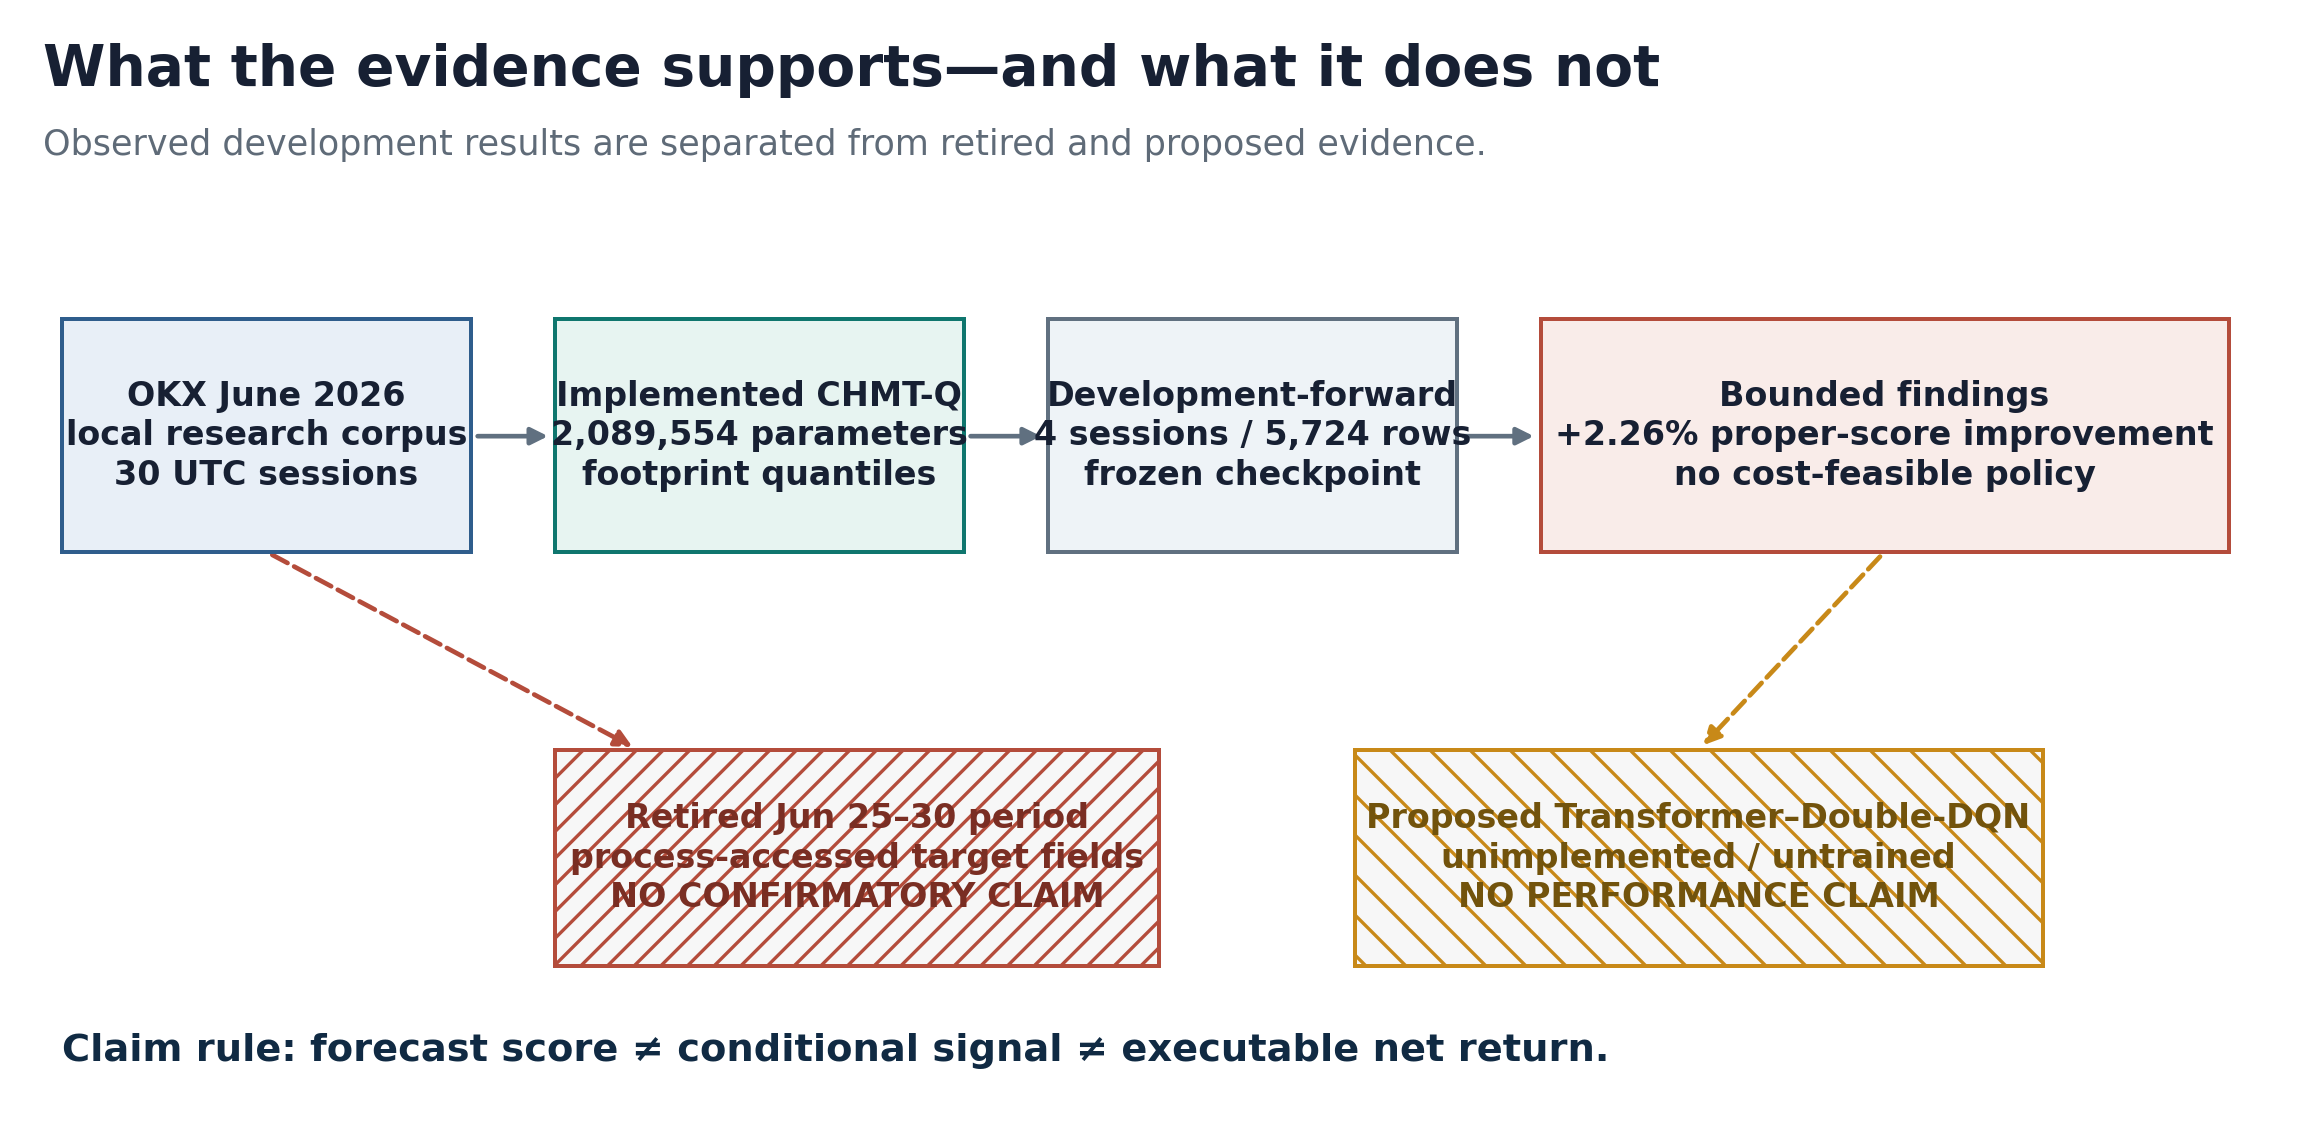
\includegraphics[width=0.94\textwidth]{assets/evidence_map.png}
\caption{Evidence and claim boundary. Only frozen development artifacts support
the reported findings. The process-accessed retired period and the proposed
reinforcement-learning study support no performance claim.}
\label{fig:evidence-map}
\end{figure}

\section{Related Work}

\subsection{Order-book representation and multi-horizon prediction}

DeepLOB established a convolutional-recurrent baseline for extracting spatial
and temporal structure from limit-order-book tensors \citep{deepLOB2019}.
Subsequent studies used attention and Transformers for order books
\citep{wallbridge2020,zhang2021lob}, standardized prediction benchmarks
\citep{ntakaris2018}, linked order-flow imbalance to multi-horizon return
predictability \citep{kolm2023}, and showed that market, label, horizon, and
evaluation choices materially change apparent performance
\citep{lucchese2024,briola2025}. Universal price-formation evidence suggests
that some representations transfer across instruments \citep{sirignano2019},
but it does not establish that a particular target or execution rule transfers.

CHMT-Q follows the representational lesson that book rank, side, and time should
not be flattened indiscriminately. It differs in objective: it forecasts
footprint primitives rather than a direct return or trade action. That choice is
central to the result because representation quality cannot repair weak
alignment between the supervised target and the downstream decision.

\subsection{Probabilistic forecasting}

Pinball loss is a consistent score for conditional quantiles
\citep{gneiting2007}. Noncrossing parameterizations can impose ordered
quantiles, while conformal methods can calibrate intervals under explicit
exchangeability or adaptation assumptions \citep{romano2019}. CHMT-Q uses an
ordered head but makes no distribution-free coverage claim. Its reported
10\%--90\% coverage is descriptive; no conformal correction was fit on the
four-day forward partition.

The mixed record of complex time-series models against linear baselines
\citep{zeng2023} makes strong simple comparators essential. Only
empirical-marginal and zero-residual baselines were registered in this run.
The absence of ridge, boosted-tree, convolutional, and recurrent competitors
precludes an architectural superiority claim.

\subsection{Backtest validity and reinforcement learning}

Financial model selection is vulnerable to repeated testing, dependence,
nonstationarity, and costs. Reality checks, multiple-testing corrections, the
stationary bootstrap, and backtest-overfitting diagnostics address parts of the
problem \citep{white2000,politis1994,harvey2016,bailey2017}. Gap-separated
validation is relevant when observations share features or labels
\citep{racine2000}. Four forward sessions are too few for stable daily-block
inference, so this paper reports descriptive estimates rather than confirmatory
tail probabilities.

Deep Q-learning \citep{mnih2015}, Double DQN \citep{hasselt2016}, dueling
decomposition \citep{wang2016dueling}, distributional Q-learning
\citep{dabney2018}, and conservative offline objectives \citep{kumar2020}
provide tools for a future decision model. Deep reinforcement learning is
high-variance \citep{henderson2018}, and offline learning adds extrapolation
risk when candidate actions lack data support \citep{levine2020}. These methods
cannot manufacture missing information or remove transaction costs.

\section{Formal Problem and Claim Taxonomy}

\subsection{Causal information set}

\begin{definition}[Availability-causal forecast]
Let \(c\) be a decision cutoff and let every observation \(x_i\) have an
availability time \(t_i^{\mathrm{avail}}\). The legal information set is
\begin{equation}
\mathcal{F}_c =
\sigma\!\left(x_i:t_i^{\mathrm{avail}}\leq c\right).
\label{eq:filtration}
\end{equation}
A forecast is availability-causal if
\begin{equation}
\widehat{\mathbf{Y}}_{c,1:H}
= f_{\theta}\!\left(\mathcal{F}_c,\mathbf{M}_c\right),\qquad H=5,
\label{eq:forecast-map}
\end{equation}
where \(\mathbf{M}_c\) contains only fixed configuration, masks, and
normalization state permitted at cutoff \(c\).
\end{definition}

This definition concerns temporal availability, not causal identification.
The archives lack local receive timestamps and native sequence/checksum
evidence, so the implemented claim is bounded to archive event order and the
documented compiler.

\subsection{Forecast intervals and target transformation}

For cutoff \(c_i\) and one-minute interval \(\Delta\), define
\begin{equation}
I_{i,h}=[c_i+(h-1)\Delta,c_i+h\Delta),\qquad h=1,\ldots,5.
\label{eq:target-interval}
\end{equation}
Let \(P_h,P_h^{b},P_h^{s}\) denote total, buy, and sell point-of-control
prices; let \(V_h\) be eligible traded volume; let \(D_h\) be signed delta; let
\(p_{\mathrm{ref}}\) be the causal reference price; let \(\delta_p\) be tick
size; and let \(\ell_{\mathrm{ref}}\) be a causal trailing log-volume
reference. The five normalized targets are
\begin{align}
y_{h,1} &= \frac{P_h-p_{\mathrm{ref}}}{\delta_p}, &
y_{h,2} &= \frac{P_h^{b}-p_{\mathrm{ref}}}{\delta_p}, \nonumber\\
y_{h,3} &= \frac{P_h^{s}-p_{\mathrm{ref}}}{\delta_p}, &
y_{h,4} &= \log(1+V_h)-\ell_{\mathrm{ref}}, \label{eq:targets}\\
y_{h,5} &= \operatorname{clip}\!\left(\frac{D_h}{V_h},-1,1\right).
\nonumber
\end{align}
Each \((h,k)\) has an independent validity mask. Missing side-specific POC
values are undefined, not numerical zeros. These variables describe future
footprint structure; none is an executable return.

\subsection{Three evidentiary levels}

\begin{table}[!htbp]
\centering
\small
\begin{tabularx}{\textwidth}{@{}p{2.5cm}Y Y Y@{}}
\toprule
\textbf{Claim level} & \textbf{Registered question} &
\textbf{Evidence} & \textbf{Defensible conclusion}\\
\midrule
Forecast distribution & Is weighted normalized pinball below the empirical
marginal baseline? & 5,724 development-forward examples &
Yes, by 2.26\% on this partition.\\
Conditional signal & Are five-minute medians and intervals sufficiently
selective? & MAE, correlations, sign metrics, dispersion, interval width &
Weak location signal; every interval crosses zero.\\
Economic value & Does a frozen rule retain positive return after costs? &
Frictionless and fixed-bps simulations & No under the tested assumptions.\\
Generalization & Does performance persist across regimes, seeds, venues, or
instruments? & One month, one instrument, one venue, one seed, one fold &
Not established.\\
Deployment & Is the model executable in a live terminal? & Offline model and
replay artifacts & Not established; no live integration.\\
\bottomrule
\end{tabularx}
\caption{Claim taxonomy. Evidence at one level does not automatically support
the next.}
\label{tab:claims}
\end{table}

\begin{proposition}[A better target score need not create decision value]
Let \(Y\) be the supervised target, \(R\) an executable return, and \(X\) the
available state. If a model improves a proper score for
\(\mathcal{L}(Y\mid X)\), but \(R\perp Y\mid X\) and the policy-relevant part of
\(\mathcal{L}(R\mid X)\) is unchanged, the improvement creates no necessary
increase in optimal trading value.
\end{proposition}

\begin{proof}
For any action \(a\) and cost \(C(a,X)\), conditional decision value is
\begin{equation}
V(a\mid X)=\E[aR-C(a,X)\mid X].
\label{eq:decision-value}
\end{equation}
The score for \(Y\) does not occur in this expression. Conditional independence
gives \(\E[R\mid X,Y]=\E[R\mid X]\), so a more accurate representation of
\(\mathcal{L}(Y\mid X)\) leaves every \(V(a\mid X)\) unchanged unless it also
changes information about \(R\), the action map, or costs. As a concrete
counterexample, take \(Y=X+\epsilon\) and \(R=\eta\), where
\(\epsilon,\eta\) are independent, centered noises. A model using \(X\) beats a
marginal forecast for \(Y\), while every nonzero trade has zero expected gross
return and negative expected net return under positive costs.
\end{proof}

\section{Data, Partitions, and Integrity Boundary}

\subsection{Source and provenance}

The source corpus comprises official OKX historical archives for BTC-USDT spot
for June 2026 UTC: 31 level-2 files and 31 trade files containing 149,390,769
raw level-2 records and 16,918,630 trades. Compilation produced 42,930 examples
across 30 UTC sessions in 168 Arrow shards (1.612 GiB). The immutable dataset
identifier is
\code{565c1d8e912ee426a1a92572d5be481ec5168d54d1ae53bd77fdd70d888e4df6}.

The corpus lacks local receive timestamps, native sequence numbers, and
checksums; June-effective instrument metadata was not independently verified;
and the license/provenance review was incomplete. The data owner authorized
local, non-promotable research subject to those limitations. The paper makes no
claim about live receive-time causality, packet-loss reconstruction, or
redistribution rights.

\subsection{Chronological split and retired period}

\begin{table}[!htbp]
\centering
\begin{tabular}{@{}lrrl@{}}
\toprule
\textbf{Partition} & \textbf{Sessions} & \textbf{Examples} & \textbf{Role}\\
\midrule
Training & 18 & 25,758 & Parameter fitting\\
Selection & 2 & 2,862 & Checkpoint selection\\
Development-forward & 4 & 5,724 & Reported evaluation\\
Retired final period & 6 & 8,586 & No confirmatory use\\
\bottomrule
\end{tabular}
\caption{Frozen chronological partition.}
\label{tab:partition}
\end{table}

\begin{figure}[!htbp]
\centering
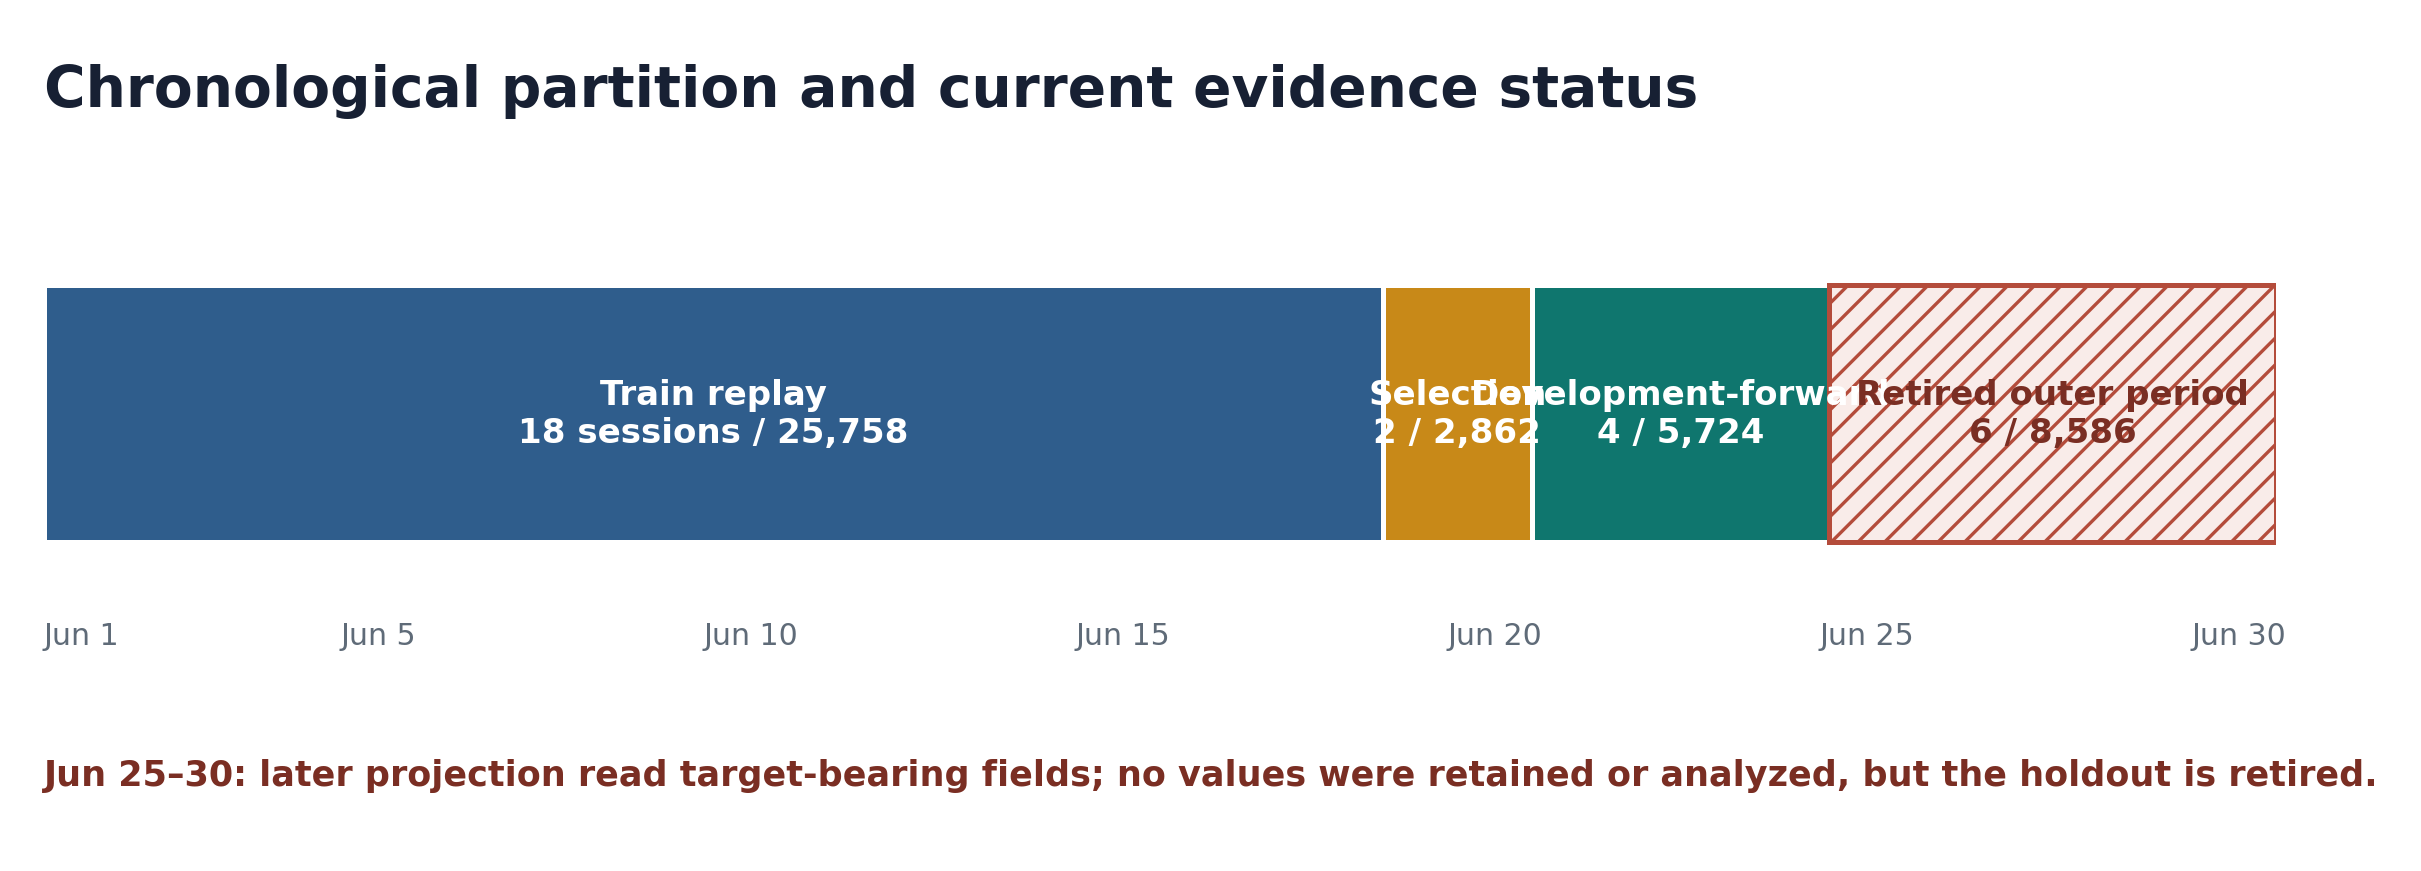
\includegraphics[width=0.93\textwidth]{assets/study_timeline.png}
\caption{Chronological evidence partition. A later schema/count projection
physically read target-bearing fields in the final six sessions, so that period
is process-accessed and retired from confirmatory use.}
\label{fig:timeline}
\end{figure}

The final 8,586 examples were not scored in the historical study. Later, a
schema/count projection traversed all 42,930 rows and physically read projected
target fields in those shards. No values were printed, retained, analyzed, or
used. Nevertheless, physical access violates a strict holdout-control policy.
The period is therefore not described as sealed, untouched, or confirmatory.
A future study requires a newly acquired, access-controlled holdout.

\subsection{Evaluation protocol}

The selected checkpoint came from epoch 10, optimizer step 2,010. Predictions
were made once per minute. Economic decisions were sampled every five minutes;
the proxy entered at the next minute open and exited at the close four minutes
later. Notional was fixed; leverage, pyramiding, endogenous impact, queue
position, and partial fills were excluded. Cost scenarios were 0, 9, 12, or 20
basis points per side, with 12 bps designated as the base case.

The registered forecast endpoint was weighted normalized pinball loss against
an empirical marginal forecast fit only on permitted data. The registered
economic rule was interval-based long-flat selection. Median-sign long-flat
and long-short rules were post hoc diagnostics. A 10,000-replicate daily-block
bootstrap was computed, but four forward days are too few for stable
confirmatory inference.

\section{CHMT-Q Architecture}

\begin{figure}[!htbp]
\centering
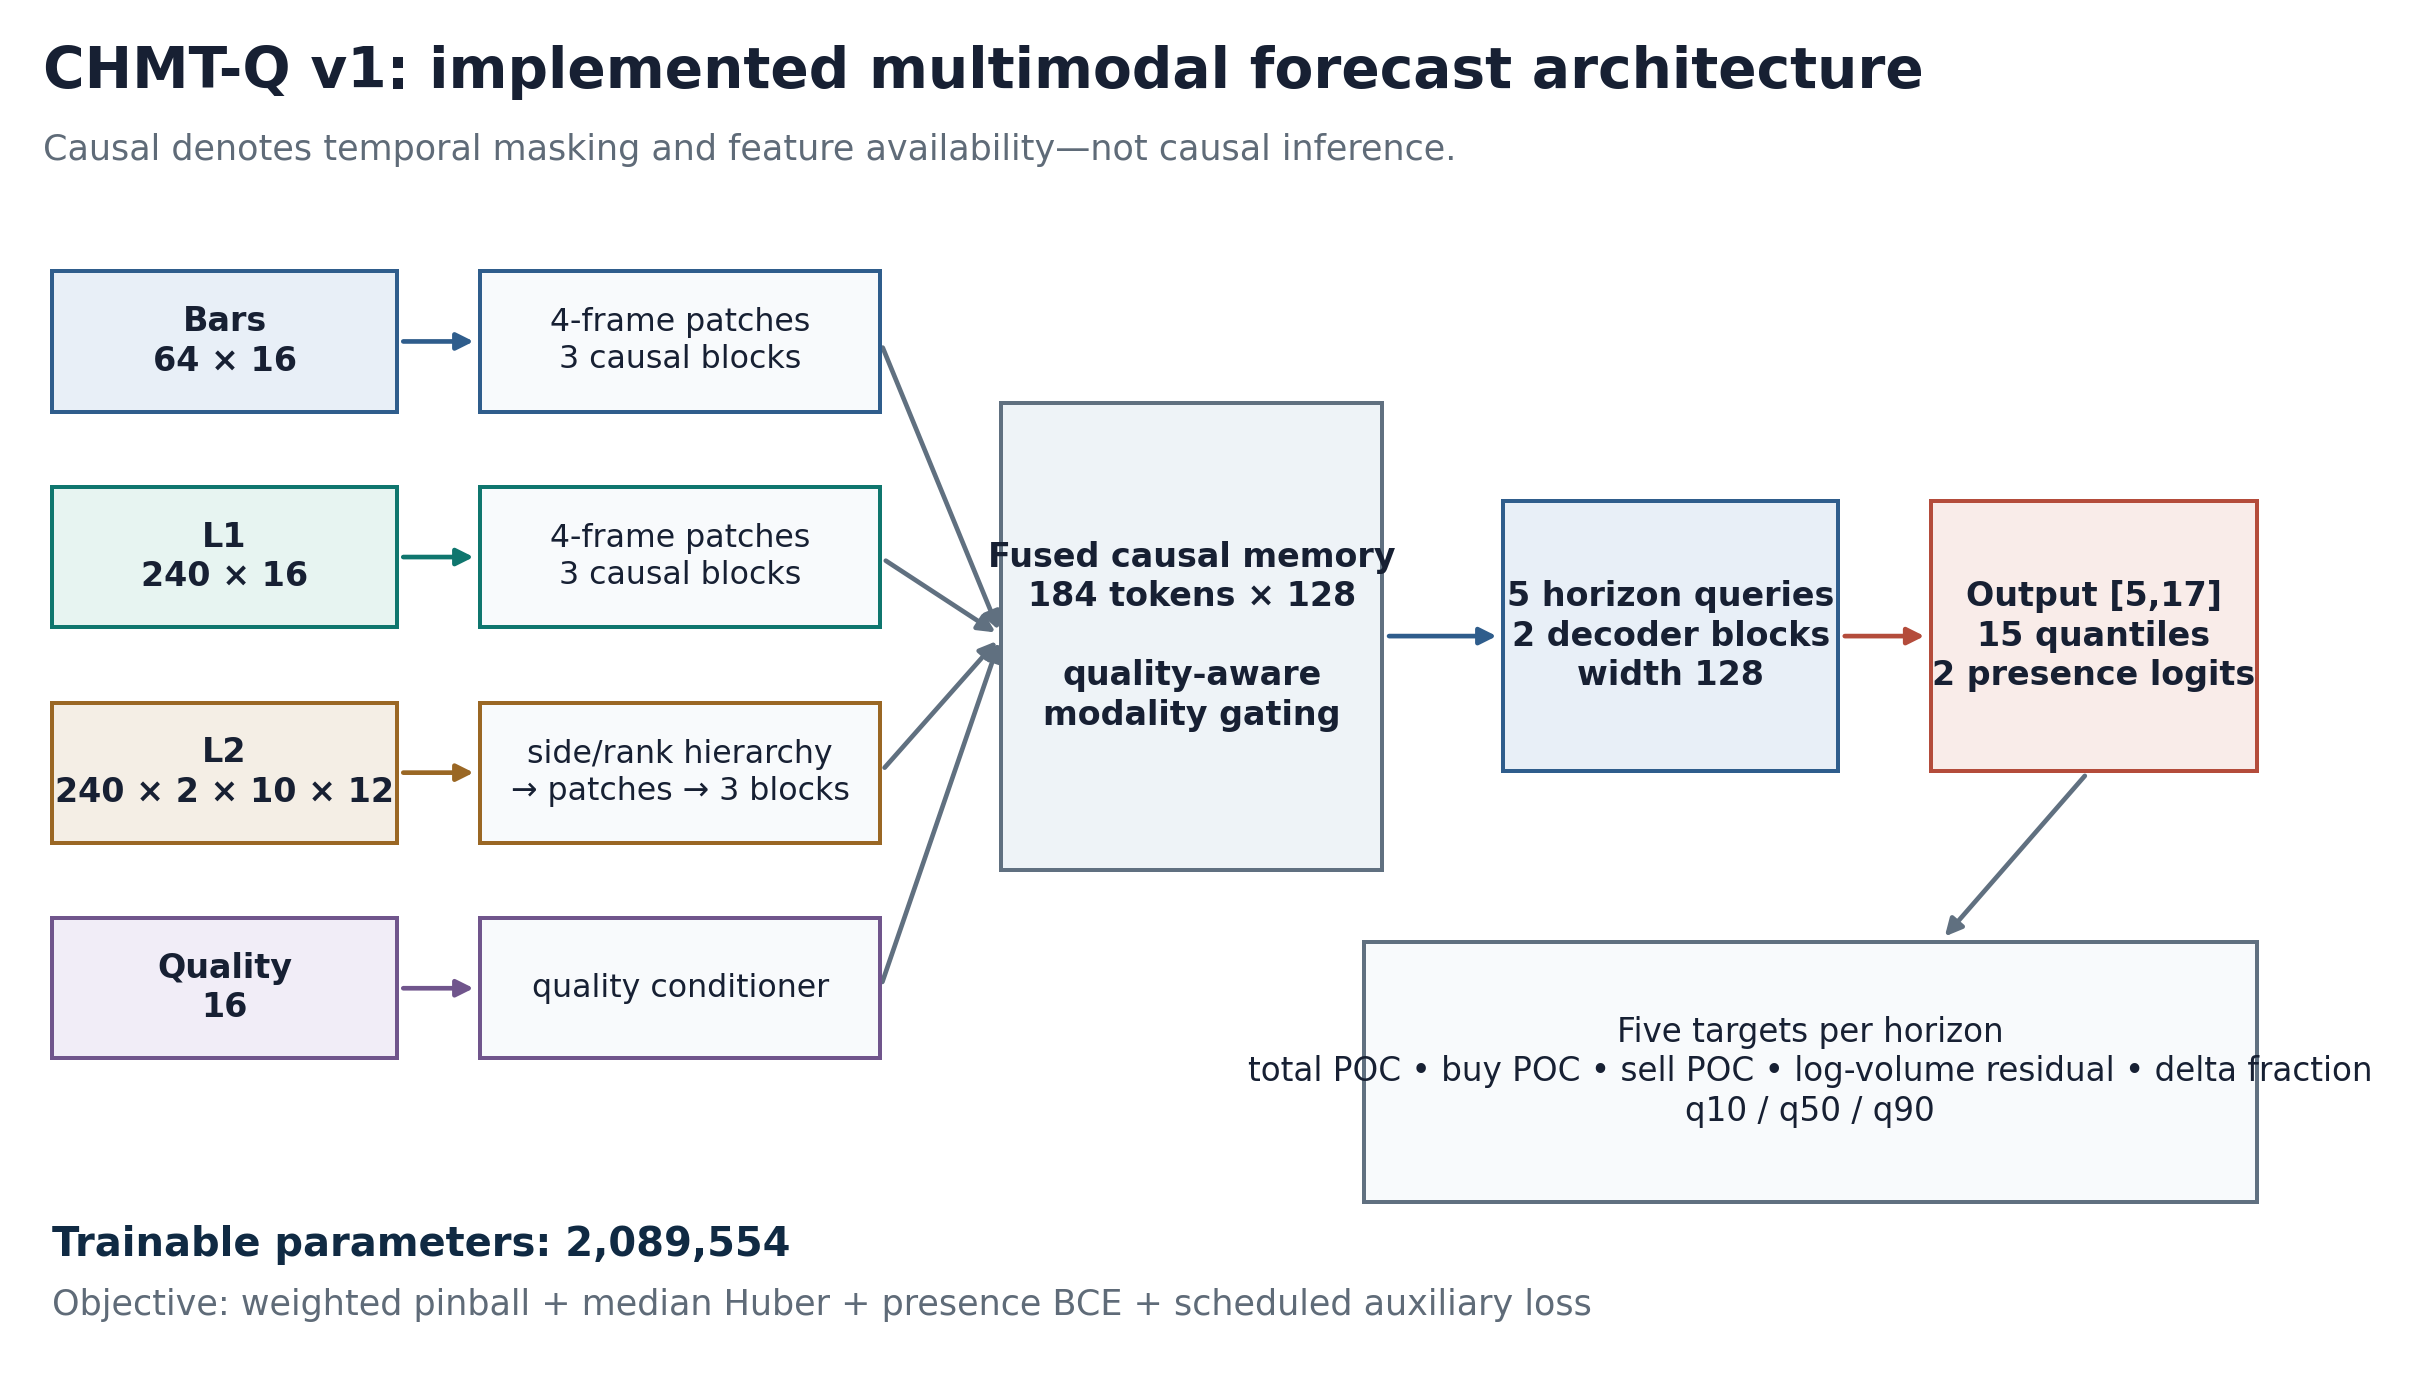
\includegraphics[width=0.94\textwidth]{assets/architecture.png}
\caption{Implemented CHMT-Q architecture. Book rank is encoded before time;
bar, L1, and L2 memories are fused with quality context and decoded by five
horizon queries.}
\label{fig:architecture}
\end{figure}

\subsection{Tensor contract and shape trace}

For batch size \(B\), inputs are
\begin{equation}
\mathbf{X}^{b}\in\R^{B\times64\times16},\quad
\mathbf{X}^{1}\in\R^{B\times240\times16},\quad
\mathbf{X}^{2}\in\R^{B\times240\times2\times10\times12},\quad
\mathbf{q}\in\R^{B\times16}.
\label{eq:inputs}
\end{equation}
Level-1 and level-2 span 120 seconds at nominal half-second resolution. Four
microstructure frames are pooled into one two-second patch, yielding 60 tokens
for each fast modality. Bars retain 64 one-minute tokens. The fused memory has
\(64+60+60=184\) tokens of width 128. Five learned horizon queries produce a
raw tensor in \(\R^{B\times5\times17}\): 15 values parameterize three
quantiles for five targets and two logits represent buy/sell presence.

\begin{table}[!htbp]
\centering
\small
\begin{tabularx}{\textwidth}{@{}Y Y Y@{}}
\toprule
\textbf{Component} & \textbf{External / internal shape} &
\textbf{Implemented setting}\\
\midrule
Bars & \(64\times16\rightarrow64\times128\) & 3 causal blocks\\
Level 1 & \(240\times16\rightarrow60\times128\) &
4-frame patch; 3 causal blocks\\
Level 2 & \(240\times2\times10\times12
\rightarrow240\times20\times32\rightarrow60\times128\) &
1 rank-side block; 3 temporal blocks\\
Quality & \(16\rightarrow128\) & Three hard-aware modality gates\\
Main attention & width 128, 4 heads & head width 32; FFN width 256\\
Level attention & width 32, 4 heads & head width 8; FFN width 64\\
Decoder & \(5\times128\) & 2 blocks; 184-token cross-attention\\
Output & \(5\times17\) & \(5\times3\) quantiles + 2 logits per horizon\\
Parameters & scalar total & 2,089,554 trainable\\
\bottomrule
\end{tabularx}
\caption{Implemented tensor and architecture contract.}
\label{tab:architecture}
\end{table}

\subsection{Causal robust scaling and physical-time encoding}

For feature \(j\), the training-only robust scale and transformed value are
\begin{equation}
s_j=\max\!\left(1.4826\,\operatorname{MAD}_{\mathrm{train},j},10^{-6}\right),
\qquad
z_j=\operatorname{clip}\!\left(\frac{x_j-\mu_j}{s_j},-8,8\right).
\label{eq:robust-scale}
\end{equation}
Invalid rows are zeroed after scaling; masks remain authoritative.

For nonnegative age \(a\), maximum age \(a_{\max}\), and fixed scales
\(\{\tau_k\}_{k=1}^{K}\), define
\begin{equation}
\phi(a)=\left[
\frac{a}{a_{\max}},
\frac{\log(1+a)}{\log(1+a_{\max})},
\sin\frac{a}{\tau_1},\cos\frac{a}{\tau_1},\ldots,
\sin\frac{a}{\tau_K},\cos\frac{a}{\tau_K}
\right],
\label{eq:time-features}
\end{equation}
and
\begin{equation}
e_t(a)=W_2\operatorname{SiLU}(W_1\phi(a)+b_1)+b_2.
\label{eq:time-mlp}
\end{equation}
Bars use scales 60 through 3,840 seconds; microstructure uses scales 0.5
through 64 seconds. L2 tokens also receive learned side and rank embeddings:
\begin{equation}
x_{t,s,r}^{(0)}
=W_{\mathrm{level}}z_{t,s,r}+e^{\mathrm{side}}_s+e^{\mathrm{rank}}_r.
\label{eq:l2-embedding}
\end{equation}

Temporal attention head \(j\) uses a learned nonnegative recency coefficient:
\begin{equation}
b_{i\ell}^{(j)}
=-\softplus(\gamma_j)\log\!\left(
1+\frac{t_i-t_\ell}{s_m}\right),\qquad t_\ell\leq t_i,
\label{eq:relative-bias}
\end{equation}
where \(s_m=60\) seconds for bars and \(s_m=2\) seconds for patched
microstructure. This is a learned bias, not a hard decay.

\subsection{Custom attention block}

For width \(d\), gain \(g\), and \(\epsilon>0\), RMSNorm
\citep{zhang2019rms} is
\begin{equation}
\RMSNorm(x)=g\odot
\frac{x}{\sqrt{d^{-1}\sum_{k=1}^{d}x_k^2+\epsilon}}.
\label{eq:rmsnorm}
\end{equation}
For head \(j\), normalized states \(U\), and memory \(M\),
\begin{equation}
Q_j=UW_j^Q,\qquad K_j=MW_j^K,\qquad V_j=MW_j^V.
\label{eq:qkv}
\end{equation}
Each query and key vector is root-mean-square normalized:
\begin{equation}
\bar q=\frac{q}{\sqrt{d_h^{-1}\lVert q\rVert_2^2+\epsilon}},
\qquad
\bar k=\frac{k}{\sqrt{d_h^{-1}\lVert k\rVert_2^2+\epsilon}}.
\label{eq:qk-norm}
\end{equation}
With learned log-temperature \(\theta_j\), optional time bias
\(b_{i\ell}^{(j)}\), modality log-gate bias \(g^{(m(\ell))}\), and eligibility
mask \(\mathcal{M}_{i\ell}\), the score is
\begin{equation}
s_{i\ell}^{(j)}
=e^{\theta_j}\frac{\bar q_i^{(j)\top}\bar k_\ell^{(j)}}{\sqrt{d_h}}
+b_{i\ell}^{(j)}+g^{(m(\ell))}+\mathcal{M}_{i\ell}.
\label{eq:attention-score}
\end{equation}

For eligibility indicator \(m_{i\ell}\), let
\(a_i=\bigvee_\ell m_{i\ell}\) and
\(r_{i\ell}=m_{i\ell}\exp(s_{i\ell}-s_i^{\max})\), with the maximum taken
only over eligible keys. Safe masked softmax is
\begin{equation}
p_{i\ell}=
\begin{cases}
r_{i\ell}/\sum_k r_{ik},&a_i=1,\\
0,&a_i=0.
\end{cases}
\label{eq:safe-softmax}
\end{equation}
This explicit zero branch prevents NaN output when every key is masked.
Multi-head output and the SwiGLU feed-forward sublayer
\citep{shazeer2020} are
\begin{align}
O&=\operatorname{Concat}_j(P_jV_j)W^O+b^O, \label{eq:attention-output}\\
\operatorname{FFN}(x)
&=W_o\!\left[
\operatorname{SiLU}(W_gx+b_g)\odot(W_ux+b_u)
\right]+b_o. \label{eq:swiglu}
\end{align}
Pre-norm LayerScale residual updates are
\begin{align}
u&=x+\lambda_a\odot
\operatorname{Dropout}(\operatorname{Attention}(\RMSNorm(x))),\nonumber\\
z&=u+\lambda_f\odot
\operatorname{Dropout}(\operatorname{FFN}(\RMSNorm(u))).
\label{eq:residual}
\end{align}
Invalid query rows are zeroed after the update.

\subsection{Causal patching and hierarchical level encoding}

For four projected L1 or L2 frame states \(x_j\) with masks \(m_j\), the
learned patch pool is
\begin{align}
r_j&=w_2^\top\tanh(W_1x_j+b_1)+b_2,\qquad j=0,\ldots,3,\nonumber\\
\pi_j&=\SafeSoftmax_j(r_j;m_j),\qquad
p=\sum_{j=0}^{3}\pi_jx_j.
\label{eq:patch-pool}
\end{align}
An all-invalid patch returns zero and an invalid mask.

Within one L2 snapshot, 20 bid/ask rank positions coexist at the same time, so
the level block is masked but not temporally triangular. A learned book query
pools level states:
\begin{align}
a_{s,r}
&=\SafeSoftmax_{s,r}\!\left(
\frac{q_{\mathrm{book}}^\top\RMSNorm(x_{s,r})}{\sqrt{32}};m_{s,r}
\right),\nonumber\\
d_t&=W_d\sum_{s,r}a_{s,r}x_{t,s,r}+b_d\in\R^{128}.
\label{eq:book-pool}
\end{align}
The resulting 240 depth-frame tokens are patched to 60 and processed by three
causal temporal blocks. This rank-before-time hierarchy separates same-snapshot
book geometry from temporal evolution.

\subsection{Quality-aware fusion and direct decoder}

Let \(s_b,s_1,s_2\) be the latest valid summaries, \(c_q\) the quality-MLP
output, and \(a_m\in\{0,1\}\) a hard modality-availability indicator. For each
modality,
\begin{align}
\widetilde g_m&=a_m\,\sigmoid\!\left(
w_{m,2}^{\top}\operatorname{SiLU}
(W_{m,1}[s_m;c_q]+b_{m,1})+b_{m,2}\right),\nonumber\\
\alpha_m&=\frac{\widetilde g_m}{\sum_n\widetilde g_n+\epsilon},\qquad
c=\RMSNorm\!\left(c_q+\sum_m\alpha_ms_m\right).
\label{eq:fusion-gates}
\end{align}
Encoded histories concatenate to
\begin{equation}
M=[M_b;M_1;M_2]\in\R^{B\times184\times128}.
\label{eq:fused-memory}
\end{equation}
The decoder receives \(\log(\alpha_m+\epsilon)\) as a key-modality score bias;
hard-masked modalities cannot be revived by a learned gate.

For horizon \(h\in\{1,\ldots,5\}\) and forecast interval \(\Delta=60\) seconds,
the initial query is
\begin{equation}
q_h^{(0)}=e_h+W_c\,c+
\operatorname{HorizonMLP}\!\left[h/5,\log(1+h),h\Delta\right].
\label{eq:horizon-query}
\end{equation}
Two decoder blocks perform horizon self-attention, cross-attention to \(M\),
and SwiGLU updates. Horizon self-attention is noncausal because all five
queries are formed at the same decision cutoff. No predicted horizon is fed
into another.

\subsection{Ordered quantile head}

For each horizon-target pair, the head produces a center \(c\) and gap logits
\(a,b\):
\begin{equation}
\widehat Q_{0.50}=c,\qquad
\widehat Q_{0.10}=c-\softplus(a),\qquad
\widehat Q_{0.90}=c+\softplus(b).
\label{eq:ordered-head}
\end{equation}
Because \(\softplus(x)=\log(1+e^x)>0\), the outputs satisfy
\(\widehat Q_{0.10}\leq\widehat Q_{0.50}\leq\widehat Q_{0.90}\).
For delta fraction, the monotone map \(\tanh\) preserves this order while
restricting each marginal to \([-1,1]\). Applying a saturating bounded map
after gap construction can, however, collapse tail resolution; empirically,
the lower delta quantile was near \(-1\) in all forward cases and the upper
quantile near \(+1\) in 78.0\%.

Physical reconstruction is
\begin{align}
\widehat P&=p_{\mathrm{ref}}+\delta_p\widehat y_{\mathrm{POC}},\nonumber\\
\widehat V&=\max\!\left(0,
\exp(\ell_{\mathrm{ref}}+\widehat y_V)-1\right),\nonumber\\
\widehat f_D&=\tanh(\widehat y_D).
\label{eq:inverse-targets}
\end{align}
The five-horizon output comprises marginal distributions, not a coherent joint
sample path. Products of separately predicted volume and delta-fraction
quantiles are not valid raw-delta quantiles.

\section{Training Objective and Optimization}

\subsection{Pinball loss and conditional quantiles}

For level \(\tau\in(0,1)\), residual \(u=y-q\), and forecast \(q\),
\begin{equation}
\rho_\tau(u)=u\left(\tau-\I\{u<0\}\right)
=\max\{\tau u,(\tau-1)u\}.
\label{eq:pinball}
\end{equation}

\begin{derivationbox}{Why pinball loss targets a conditional quantile}
For a conditional distribution \(F_{Y\mid X}\), define
\(R(q\mid X)=\E[\rho_\tau(Y-q)\mid X]\). Away from atoms,
\begin{align}
\frac{\partial R}{\partial q}
&=(1-\tau)\Pr(Y<q\mid X)-\tau\Pr(Y>q\mid X)\nonumber\\
&=F_{Y\mid X}(q)-\tau.
\label{eq:pinball-derivative}
\end{align}
Thus a minimum satisfies \(F_{Y\mid X}(q)=\tau\). At atoms, the subgradient
condition is \(F(q^-)\leq\tau\leq F(q)\), the standard quantile definition.
This consistency concerns \(Y\); it does not convert \(Y\) into an executable
return.
\end{derivationbox}

With horizon weights \(w_h=h^{-1/2}\), target weights
\(v=(1,1,1,0.5,0.5)\), quantiles
\(\mathcal{T}=\{0.1,0.5,0.9\}\), and validity mask \(m_{bhk}\),
\begin{equation}
\mathcal{L}_Q=
\frac{\sum_{b,h,k,\tau}m_{bhk}w_hv_k
\rho_\tau(y_{bhk}-\widehat Q_{bhk\tau})}
{\sum_{b,h,k,\tau}m_{bhk}w_hv_k+\epsilon}.
\label{eq:weighted-pinball}
\end{equation}
The longest-horizon total-POC contribution has nominal objective share
\begin{equation}
\frac{5^{-1/2}\cdot1}
{\left(\sum_{h=1}^{5}h^{-1/2}\right)
\left(\sum_{k=1}^{5}v_k\right)}
=0.034596,
\label{eq:h5-share}
\end{equation}
after the common quantile multiplicity cancels. Only 3.46\% of the
horizon-target weighting therefore directly concerns H5 total POC.

\subsection{Median, presence, and auxiliary terms}

For residual \(r\) and \(\delta=1\), Huber loss is
\begin{equation}
H_\delta(r)=
\begin{cases}
\tfrac12r^2,&|r|\leq\delta,\\
\delta(|r|-\tfrac12\delta),&|r|>\delta.
\end{cases}
\label{eq:huber}
\end{equation}
The normalized median term is
\begin{equation}
\mathcal{L}_H=
\frac{\sum_{b,h,k}m_{bhk}w_hv_k
H_\delta(y_{bhk}-\widehat Q_{bhk,0.5})}
{\sum_{b,h,k}m_{bhk}w_hv_k+\epsilon}.
\label{eq:huber-loss}
\end{equation}
For presence label \(z\in\{0,1\}\), logit \(\eta\), and presence-validity mask
\(m^P\), stable binary cross-entropy is
\begin{align}
\operatorname{BCE}(\eta,z)
&=\max(\eta,0)-\eta z+\log(1+e^{-|\eta|}),\nonumber\\
\mathcal{L}_P
&=\frac{\sum m^P\operatorname{BCE}(\eta,z)}
{\sum m^P+\epsilon}.
\label{eq:bce}
\end{align}
The final-decoder base objective is
\begin{equation}
\mathcal{L}_{\mathrm{base}}
=\mathcal{L}_Q+0.25\mathcal{L}_H+0.20\mathcal{L}_P.
\label{eq:base-loss}
\end{equation}
The same output head applied after decoder block 1 supplies a deep-supervision
term. With \(u\in[0,1]\) the fraction of planned optimizer steps,
\begin{equation}
\lambda_{\mathrm{aux}}(u)=
\begin{cases}
0.25,&u\leq0.60,\\
0.25-\dfrac{0.20}{0.30}(u-0.60),&0.60<u<0.90,\\
0.05,&u\geq0.90,
\end{cases}
\label{eq:aux-schedule}
\end{equation}
and
\begin{equation}
\mathcal{L}
=\mathcal{L}_{\mathrm{base}}^{\mathrm{final}}
+\lambda_{\mathrm{aux}}(u)
\mathcal{L}_{\mathrm{base}}^{\mathrm{aux}}.
\label{eq:total-loss}
\end{equation}
Early stopping occurred after 36\% of planned steps, so
\(\lambda_{\mathrm{aux}}=0.25\) throughout the run.

\subsection{Optimization}

The run used seed 17, AdamW with learning rate \(3\times10^{-4}\), minimum
learning rate \(3\times10^{-5}\), \((\beta_1,\beta_2)=(0.9,0.95)\),
\(\epsilon=10^{-8}\), weight decay 0.05, and 5\% warm-up. A microbatch of 32
with four-step accumulation gave an effective batch of 128. Training was
deterministic FP32 on one CUDA device. It stopped at epoch 18 after 3,618
optimizer steps and selected epoch 10 at step 2,010. If \(\mathcal{S}\) is the
set of epoch checkpoints, the frozen selection rule was
\begin{equation}
\widehat s=\arg\min_{s\in\mathcal{S}}
\mathcal{L}_{\mathrm{validation}}(\theta_s).
\label{eq:checkpoint-rule}
\end{equation}

Global norm clipping with threshold \(c=1\) maps raw gradient \(g\) to
\begin{equation}
\widetilde g=g\min\!\left(1,\frac{c}{\lVert g\rVert_2+\epsilon}\right).
\label{eq:gradient-clipping}
\end{equation}
Every recorded pre-clipping norm exceeded 1.0; the median was 19.58, the 90th
percentile 38.30, and the maximum 109.07. This proves operation in a persistently
clipped regime, but not that clipping caused the economic failure.

\begin{table}[!htbp]
\centering
\begin{tabular}{@{}lr@{}}
\toprule
\textbf{Training item} & \textbf{Value}\\
\midrule
Training / selection / forward examples & 25,758 / 2,862 / 5,724\\
Seed / folds & 1 / 1\\
Selected checkpoint & epoch 10, step 2,010\\
Final step & 3,618\\
Selected validation loss & 0.210765\\
Empirical validation baseline & 0.222446\\
Weight artifact & 8.071 MiB\\
Resumable checkpoint & 24.284 MiB\\
\bottomrule
\end{tabular}
\caption{Training and selection ledger. Validation improvement is selection
evidence, not an independent performance estimate.}
\label{tab:training}
\end{table}

\section{Evaluation Mathematics}

\subsection{Forecast baseline, score, and diagnostics}

For permitted pre-forward observations in horizon-target cell \((h,k)\), the
empirical marginal baseline is
\begin{equation}
\widehat Q^{\mathrm{emp}}_{hk\tau}
=\inf\{q:\widehat F^{\mathrm{train}}_{hk}(q)\geq\tau\}.
\label{eq:empirical-baseline}
\end{equation}
It is applied unchanged to every development-forward row. If
\(\mathcal{L}_{\mathrm{model}}\) and \(\mathcal{L}_{\mathrm{base}}\) are
Equation~\eqref{eq:weighted-pinball}, relative improvement is
\begin{equation}
\Delta_{\%}
=100\frac{\mathcal{L}_{\mathrm{base}}-\mathcal{L}_{\mathrm{model}}}
{\mathcal{L}_{\mathrm{base}}}.
\label{eq:relative-improvement}
\end{equation}

For H5 total POC, location diagnostics are
\begin{align}
\operatorname{MAE}
&=\frac{\sum_i m_i|y_i-\widehat q_i|}{\sum_i m_i},&
\operatorname{Bias}
&=\frac{\sum_i m_i(\widehat q_i-y_i)}{\sum_i m_i},\nonumber\\
r_P&=\frac{\sum_i(y_i-\bar y)(\widehat q_i-\bar q)}
{\sqrt{\sum_i(y_i-\bar y)^2\sum_i(\widehat q_i-\bar q)^2}},&
r_S&=r_P(\operatorname{rank}(y),\operatorname{rank}(\widehat q)),\nonumber\\
\kappa_\sigma&=\frac{\operatorname{sd}(\widehat q)}
{\operatorname{sd}(y)}.
\label{eq:signal-metrics}
\end{align}
For binary sign labels and predictions, Matthews correlation is
\begin{equation}
\operatorname{MCC}
=\frac{TP\cdot TN-FP\cdot FN}
{\sqrt{(TP+FP)(TP+FN)(TN+FP)(TN+FN)}}.
\label{eq:mcc}
\end{equation}
For interval \([L_i,U_i]\), empirical coverage, mean width, and zero-crossing
rate are
\begin{align}
\widehat C&=\frac{\sum_i m_i\I\{L_i\leq y_i\leq U_i\}}{\sum_i m_i},&
\widehat W&=\frac{\sum_i m_i(U_i-L_i)}{\sum_i m_i},\nonumber\\
\widehat Z&=\frac{\sum_i m_i\I\{L_i\leq0\leq U_i\}}{\sum_i m_i}.
\label{eq:interval-metrics}
\end{align}

\subsection{Decision rules and return accounting}

Let \(L_j,M_j,U_j\) be H5 total-POC lower, median, and upper forecasts. The
registered and diagnostic positions are
\begin{equation}
d_j^{\mathrm{int}}=\I\{L_j>0\},\qquad
d_j^{\mathrm{LF}}=\I\{M_j>0\},\qquad
d_j^{\mathrm{LS}}=\operatorname{sign}(M_j).
\label{eq:policies}
\end{equation}
The latter two were examined after the registered rule abstained and therefore
support diagnosis, not confirmation.

For entry \(P_j^{\mathrm{in}}\), exit \(P_j^{\mathrm{out}}\), position \(d_j\),
and one-way proportional cost \(\kappa\), the documented completed-trade
accounting is
\begin{align}
r_j^{\mathrm{gross}}
&=d_j\left(\frac{P_j^{\mathrm{out}}}{P_j^{\mathrm{in}}}-1\right),\nonumber\\
r_j^{\mathrm{net}}
&=r_j^{\mathrm{gross}}-2\kappa\,\I\{d_j\neq0\},\nonumber\\
R_{\mathrm{comp}}
&=\prod_{j=1}^{N}(1+r_j^{\mathrm{net}})-1.
\label{eq:return-accounting}
\end{align}

\begin{derivationbox}{Break-even cost}
If mean gross edge is \(e_{\mathrm{rt}}\) basis points per completed round
trip and cost is symmetric, break-even one-way cost is
\begin{equation}
\kappa_{\mathrm{BE}}=\frac{e_{\mathrm{rt}}}{2}.
\label{eq:break-even}
\end{equation}
For the long-flat diagnostic, \(e_{\mathrm{rt}}=0.4453\) bps, hence
\(\kappa_{\mathrm{BE}}=0.2227\) bps per side. The 12-bps base assumption is
\(12/0.2227=53.89\) times break-even. Equivalently, the 24-bps round-trip cost
divided by 0.4453 bps of gross edge is 53.89. This arithmetic makes the tested
turnover economically infeasible under the base cost.
\end{derivationbox}

\subsection{Dependence and descriptive block bootstrap}

At one-minute spacing, adjacent examples share
\begin{equation}
\frac{63}{64}=98.4375\%
\label{eq:bar-overlap}
\end{equation}
of bar rows. Complete five-horizon label windows share
\begin{equation}
\frac{4}{5}=80\%
\label{eq:label-overlap}
\end{equation}
of their minute intervals. A generic autocorrelation effective-sample-size
heuristic is
\begin{equation}
n_{\mathrm{eff}}
\approx\frac{n}{1+2\sum_{\ell=1}^{L}\widehat\rho(\ell)},
\label{eq:effective-n}
\end{equation}
under a stated truncation rule. The recorded H5 heuristic gave an effective
fraction near 22.3\%; this is diagnostic, not an inferential correction.

The paired daily-block bootstrap sampled four complete UTC-day blocks with
replacement, applied the same sampled blocks to model and baseline, and
recomputed
\begin{equation}
\Delta^*=\widehat{\mathcal{L}}_{\mathrm{base}}^*
-\widehat{\mathcal{L}}_{\mathrm{model}}^*.
\label{eq:block-bootstrap}
\end{equation}
With only four distinct days, its percentile distribution is descriptive and
cannot support a confirmatory p-value or broad market inference.

\section{Results}

\subsection{Aggregate probabilistic score}

On the development-forward partition,
\(\mathcal{L}_{\mathrm{model}}=0.2513909348275368\) and
\(\mathcal{L}_{\mathrm{base}}=0.25719276632184623\). Substitution into
Equation~\eqref{eq:relative-improvement} gives
\begin{equation}
100\frac{0.2571927663-0.2513909348}{0.2571927663}
=2.2558299665\%.
\label{eq:observed-improvement}
\end{equation}
This answers the distributional question positively within the bounded
development design.

\begin{figure}[!htbp]
\centering
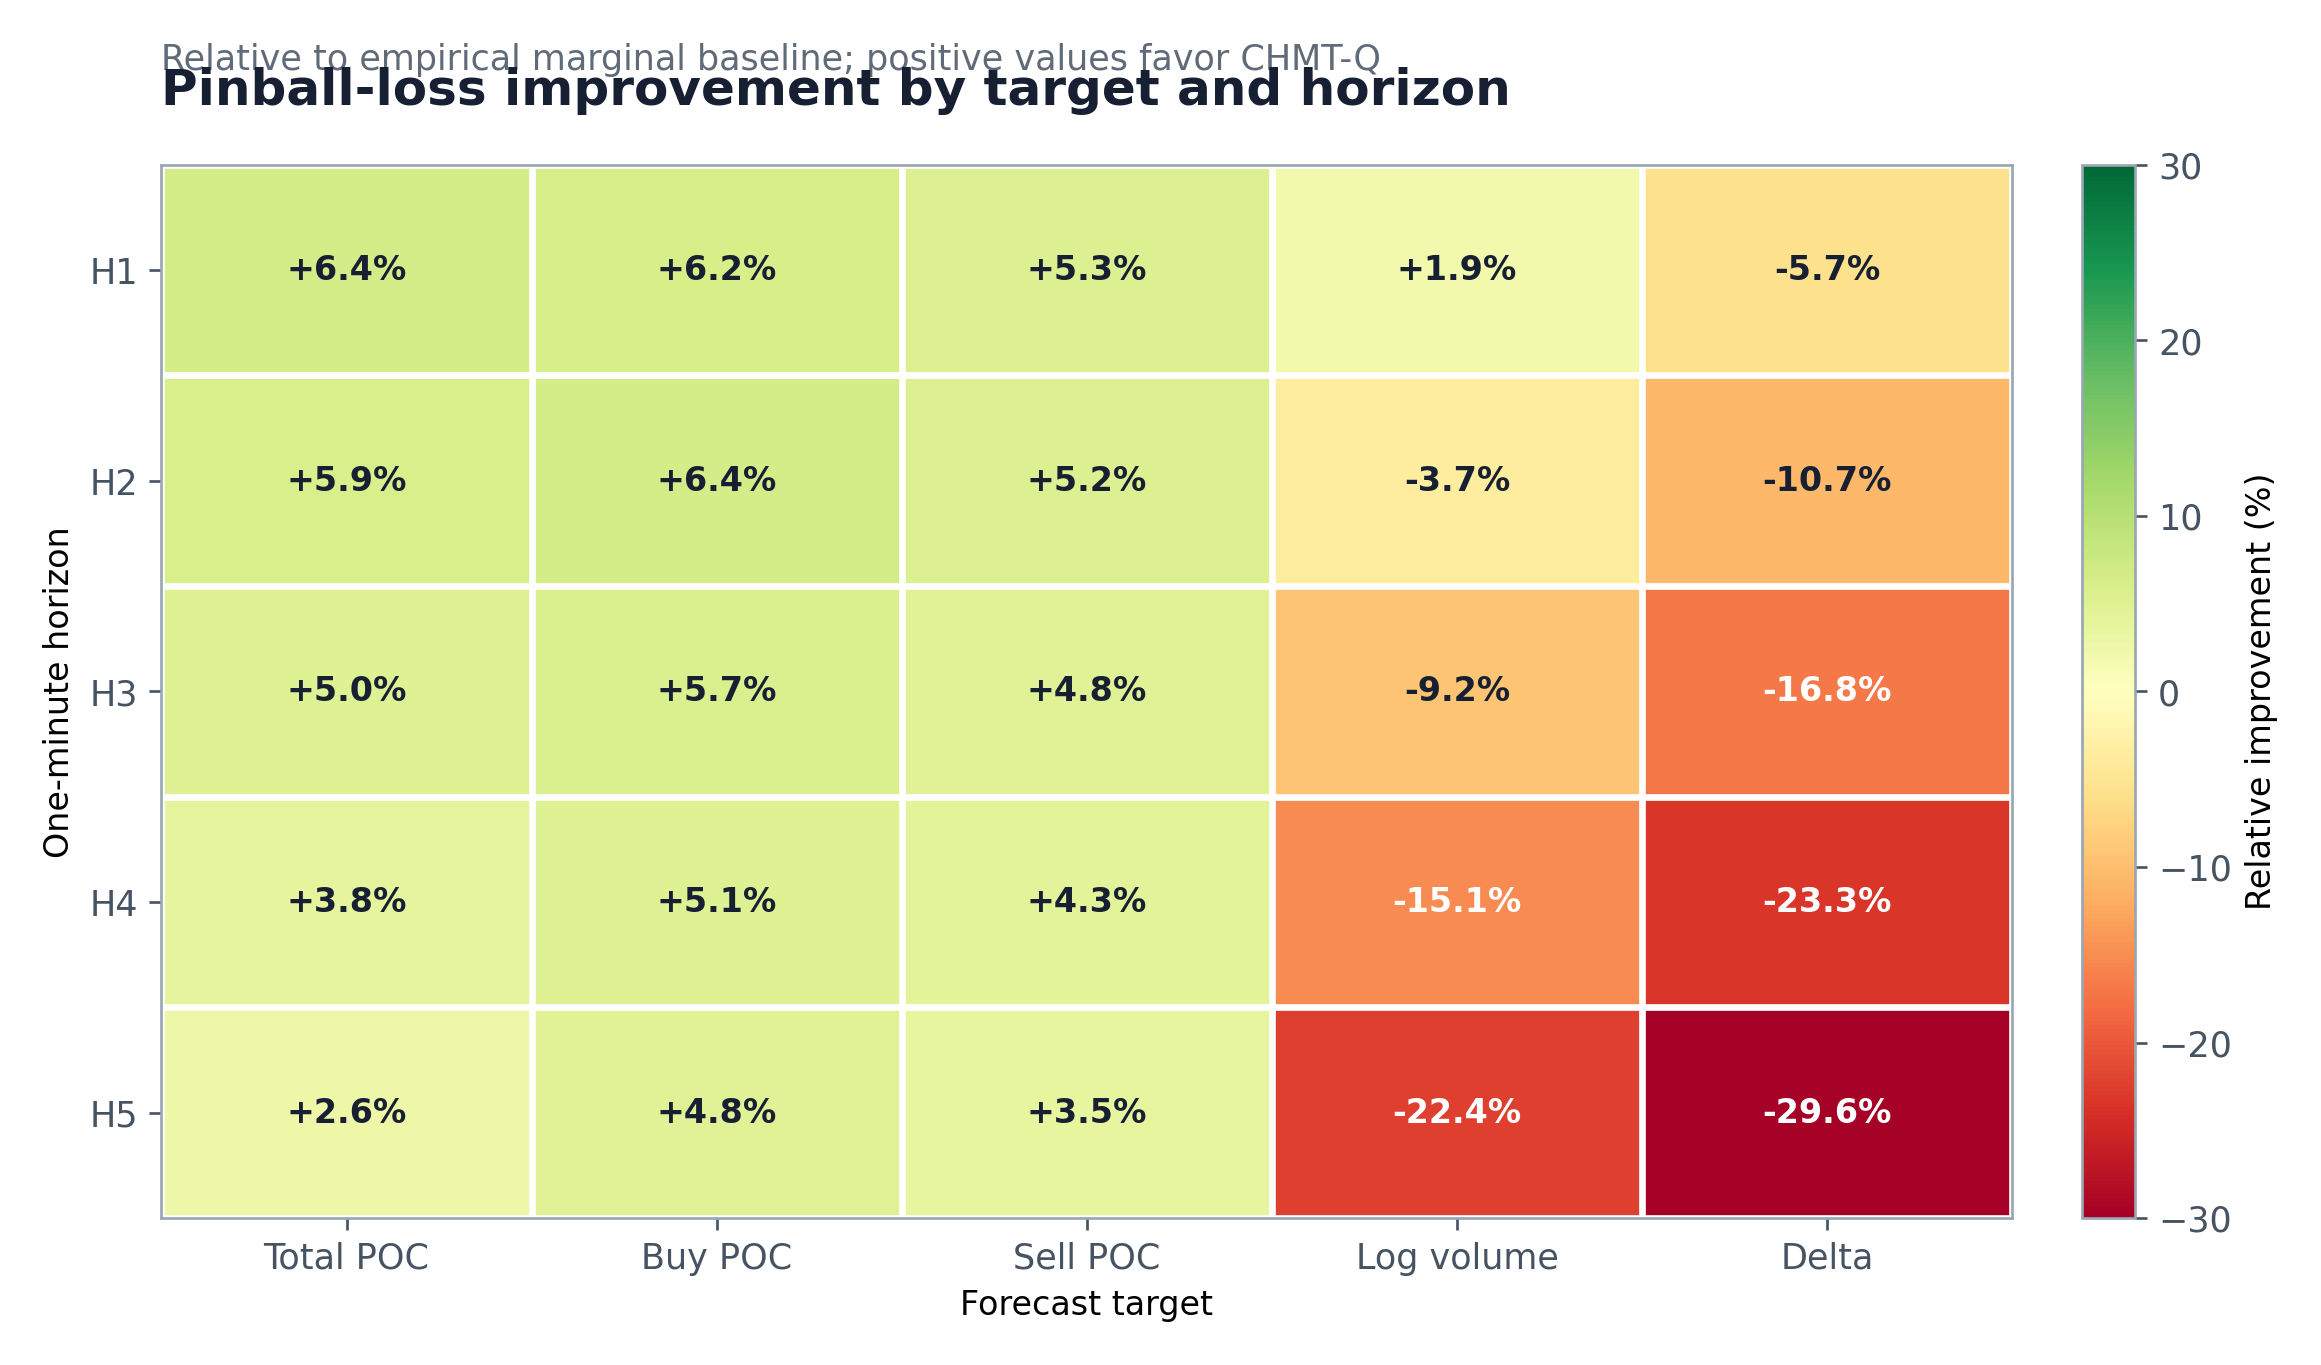
\includegraphics[width=0.86\textwidth]{assets/score_heatmap.png}
\caption{Relative pinball-loss improvement by horizon and target. Positive
values favor CHMT-Q. Aggregate weighting masks poor log-volume and delta cells.}
\label{fig:heatmap}
\end{figure}

All three POC targets improved in every horizon, with diminishing magnitude.
Log-volume residual improved only at horizon one and worsened thereafter.
Delta pinball loss was worse at every horizon. At H5, target-level relative
changes were \(+2.62\%\), \(+4.84\%\), \(+3.53\%\), \(-22.43\%\), and
\(-29.57\%\).

\begin{table}[!htbp]
\centering
\begin{tabular}{@{}lrrr@{}}
\toprule
\textbf{Forward endpoint} & \textbf{CHMT-Q} & \textbf{Baseline} &
\textbf{Relative result}\\
\midrule
Weighted normalized pinball & 0.251391 & 0.257193 & +2.2558\%\\
H5 total-POC median MAE (ticks) & 532.841 & 532.905 & +0.0119\%\\
H5 log-volume median MAE & -- & -- & 24.44\% worse\\
H5 delta median MAE & -- & -- & 44.18\% worse\\
\bottomrule
\end{tabular}
\caption{Primary forecast and selected location results. Dashes indicate that
the table reports relative diagnostics without reproducing an unused physical
unit.}
\label{tab:forecast-results}
\end{table}

The arithmetic improvement is real on this partition. It is not evidence that
a Transformer is necessary, that calibration transfers across regimes, or that
the result is statistically significant across independent market periods.

\subsection{Five-minute conditional signal}

H5 total-POC median MAE was effectively tied with the marginal baseline.
Pearson correlation was 0.0774, Spearman correlation 0.0753, and direct-sign
MCC 0.0481. A separate anchor-to-future-close direction proxy had 52.67\%
accuracy, 52.36\% balanced accuracy, MCC 0.0475, and Spearman association
0.0780.

Predicted medians had only 15.13\% of realized standard deviation. The average
10\%--90\% interval spanned 1,904.7 ticks, approximately USDT 190.47 at the
dataset tick size, and empirical coverage was 81.15\%. Every interval crossed
zero, so \(\widehat Z=1\) in Equation~\eqref{eq:interval-metrics}.

\begin{figure}[!htbp]
\centering
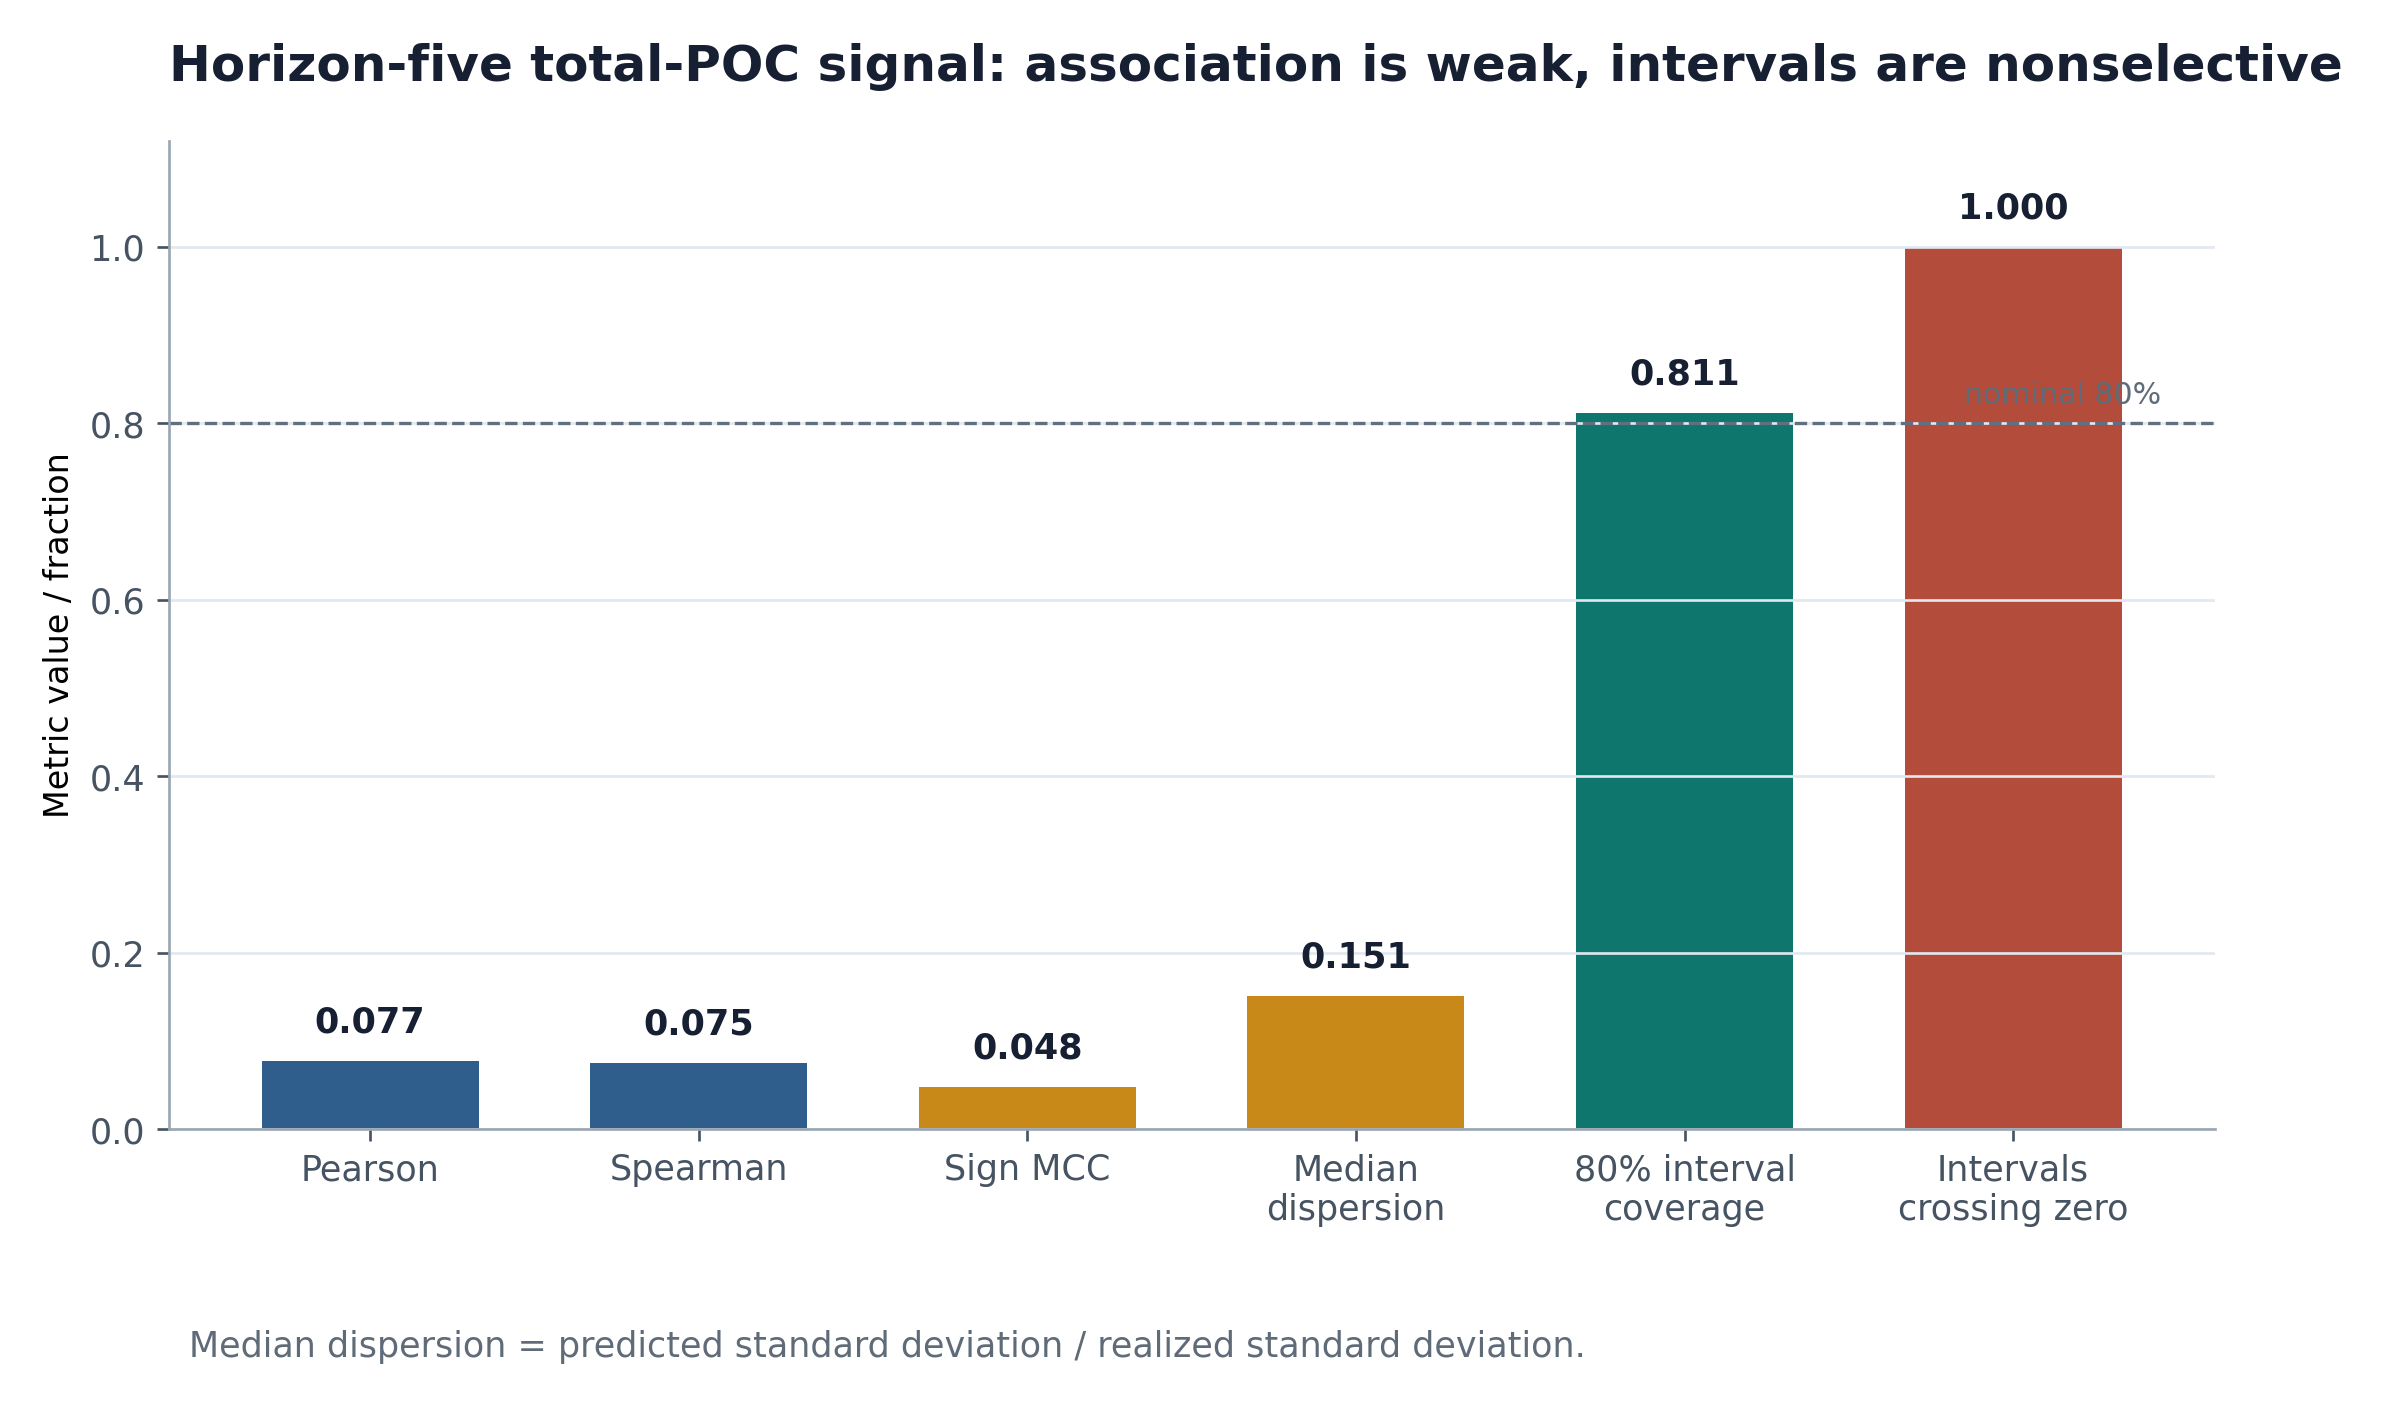
\includegraphics[width=0.86\textwidth]{assets/h5_diagnostics.png}
\caption{H5 signal diagnostics. Median association and dispersion are weak even
though nominal interval coverage is close to 80\%.}
\label{fig:h5}
\end{figure}

The coexistence of a shrunk median and broad interval is consistent with
learning marginal uncertainty more successfully than conditional location.
It does not establish useful directional selection.

\subsection{Economic feasibility}

The registered interval policy made zero trades because all intervals crossed
zero. This is not a software failure: the uncertainty-aware rule abstained.
The post hoc median-sign long-flat rule made 484 trades. Its frictionless
compounded return was \(+2.1607\%\), but its base-cost return was
\(-68.0682\%\). Mean gross edge was 0.4453 bps per round trip. The diagnostic
long-short rule made 1,148 trades, returned \(+4.989\%\) frictionlessly, and
\(-93.344\%\) at base costs; gross edge was 0.4301 bps.

\begin{table}[!htbp]
\centering
\small
\begin{tabular}{@{}lrrrc@{}}
\toprule
\textbf{Policy} & \textbf{Trades} & \textbf{Frictionless} &
\textbf{Base-cost} & \textbf{Gross bps / RT}\\
\midrule
Registered interval long-flat & 0 & 0.00\% & 0.00\% & --\\
Diagnostic median long-flat & 484 & +2.1607\% & -68.0682\% & 0.4453\\
Diagnostic median long-short & 1,148 & +4.989\% & -93.344\% & 0.4301\\
\bottomrule
\end{tabular}
\caption{Economic diagnostics. RT denotes a completed round trip.}
\label{tab:policy-results}
\end{table}

\begin{figure}[!htbp]
\centering
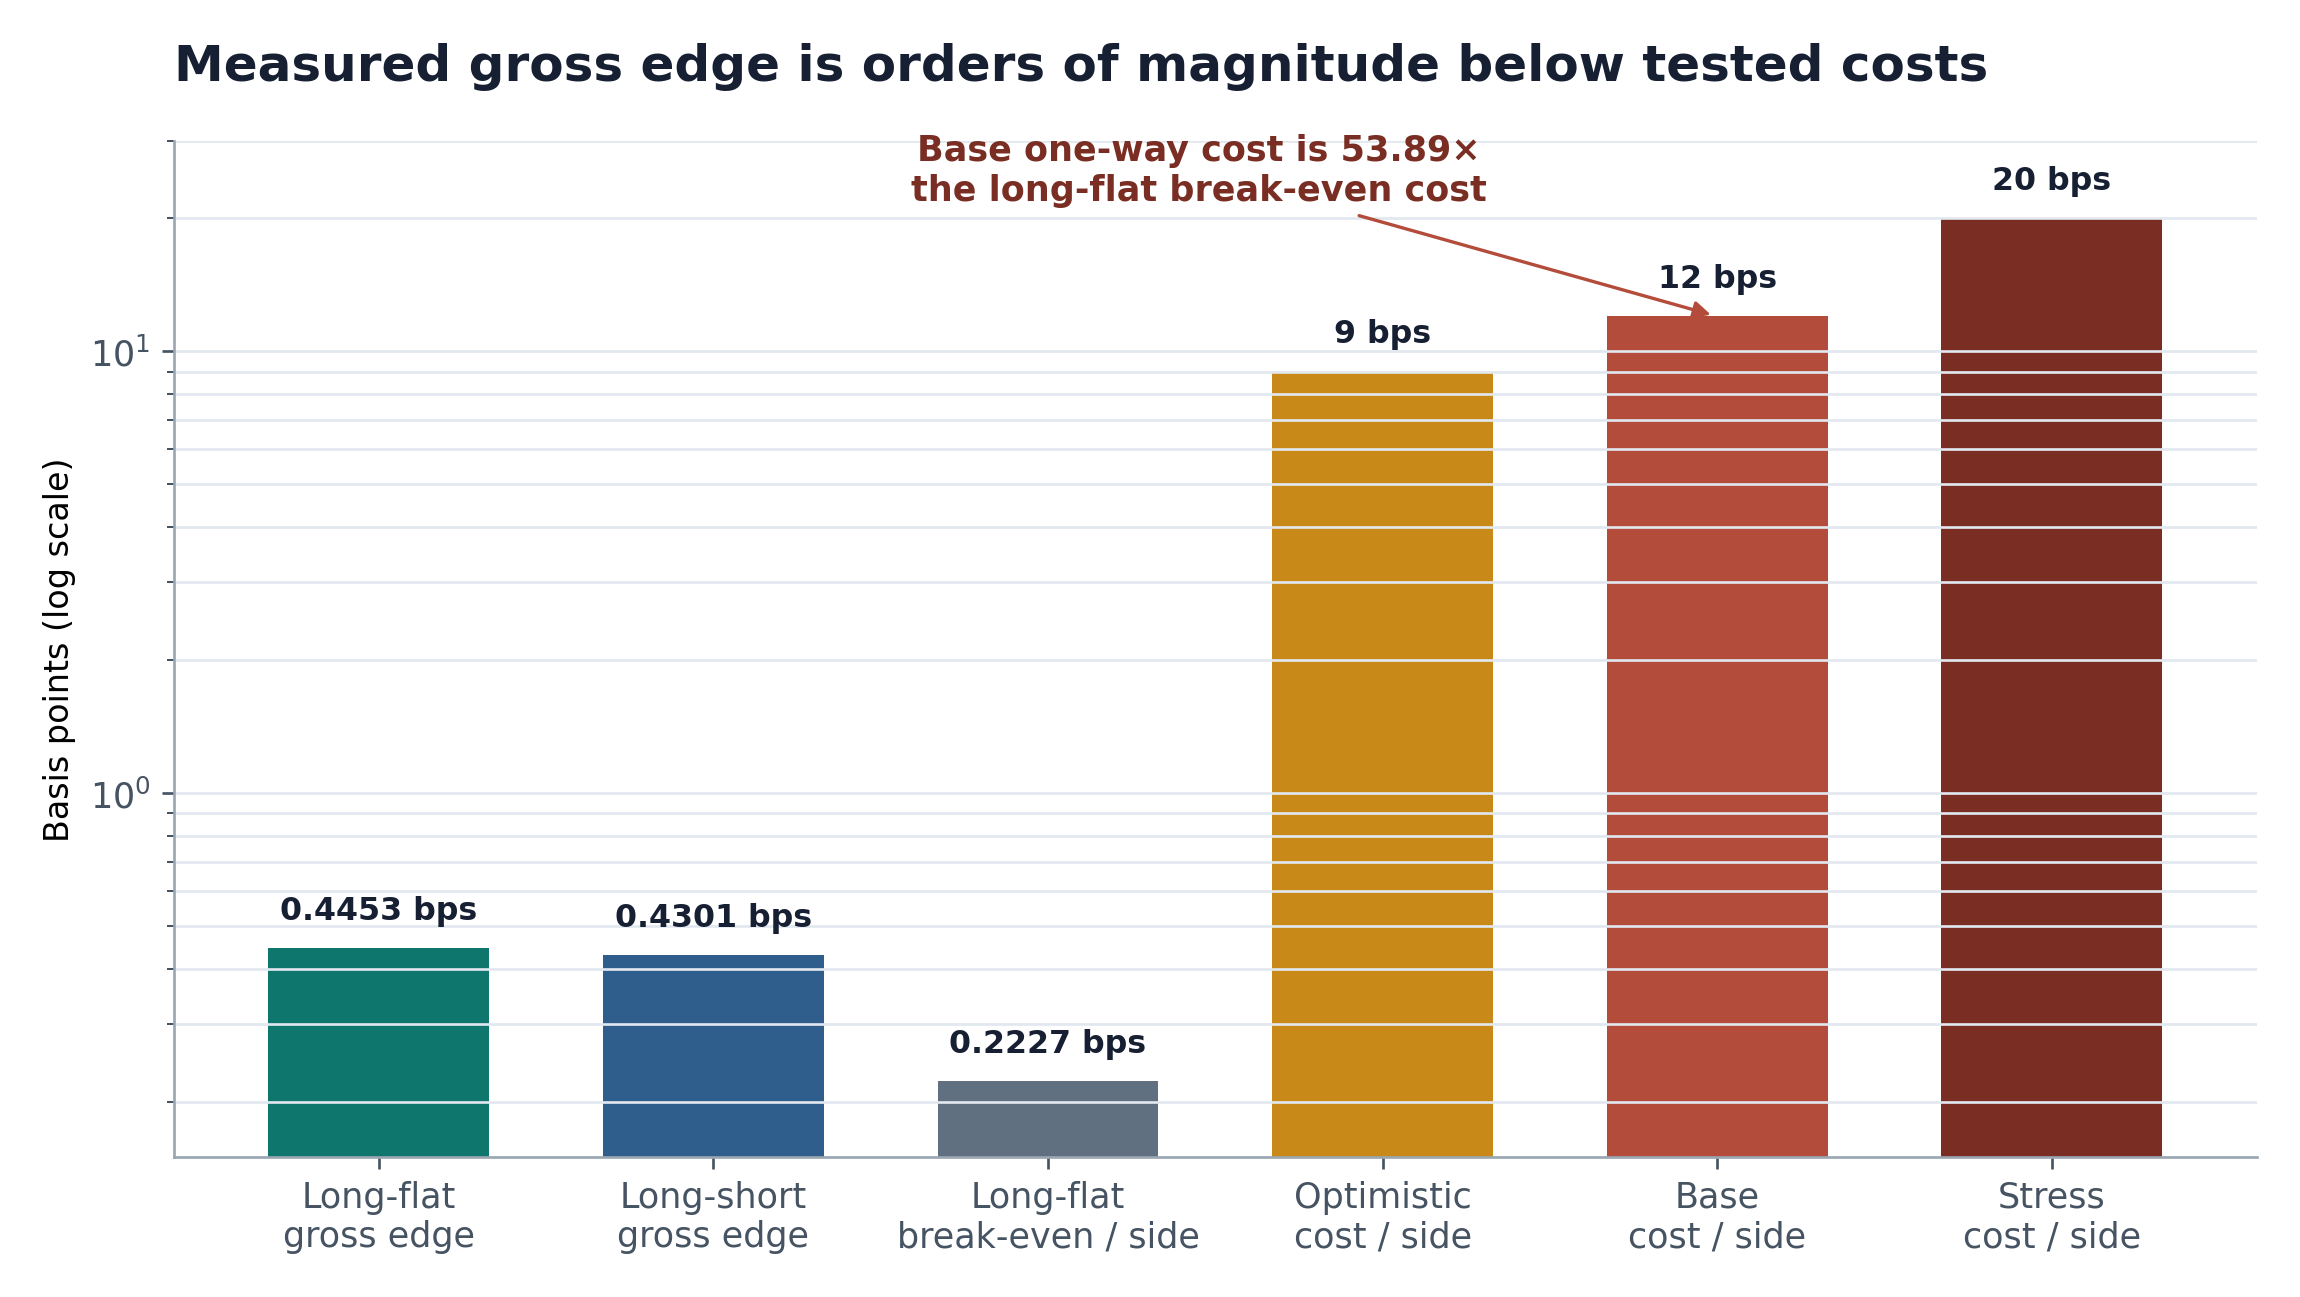
\includegraphics[width=0.86\textwidth]{assets/cost_feasibility.png}
\caption{Cost feasibility. Observed gross edge is far below the base round-trip
cost of 24 bps.}
\label{fig:costs}
\end{figure}

The simulator uses minute trade prices and fixed basis-point deductions. It
does not reproduce executable quotes, queue position, partial fills, impact,
financing, outages, or capacity. It cannot validate live profitability.
Because even this simplified accounting is cost-dominated, adding realistic
frictions would not rescue the tested policies.

\section{Failure-Factor Audit}

\begin{figure}[!htbp]
\centering
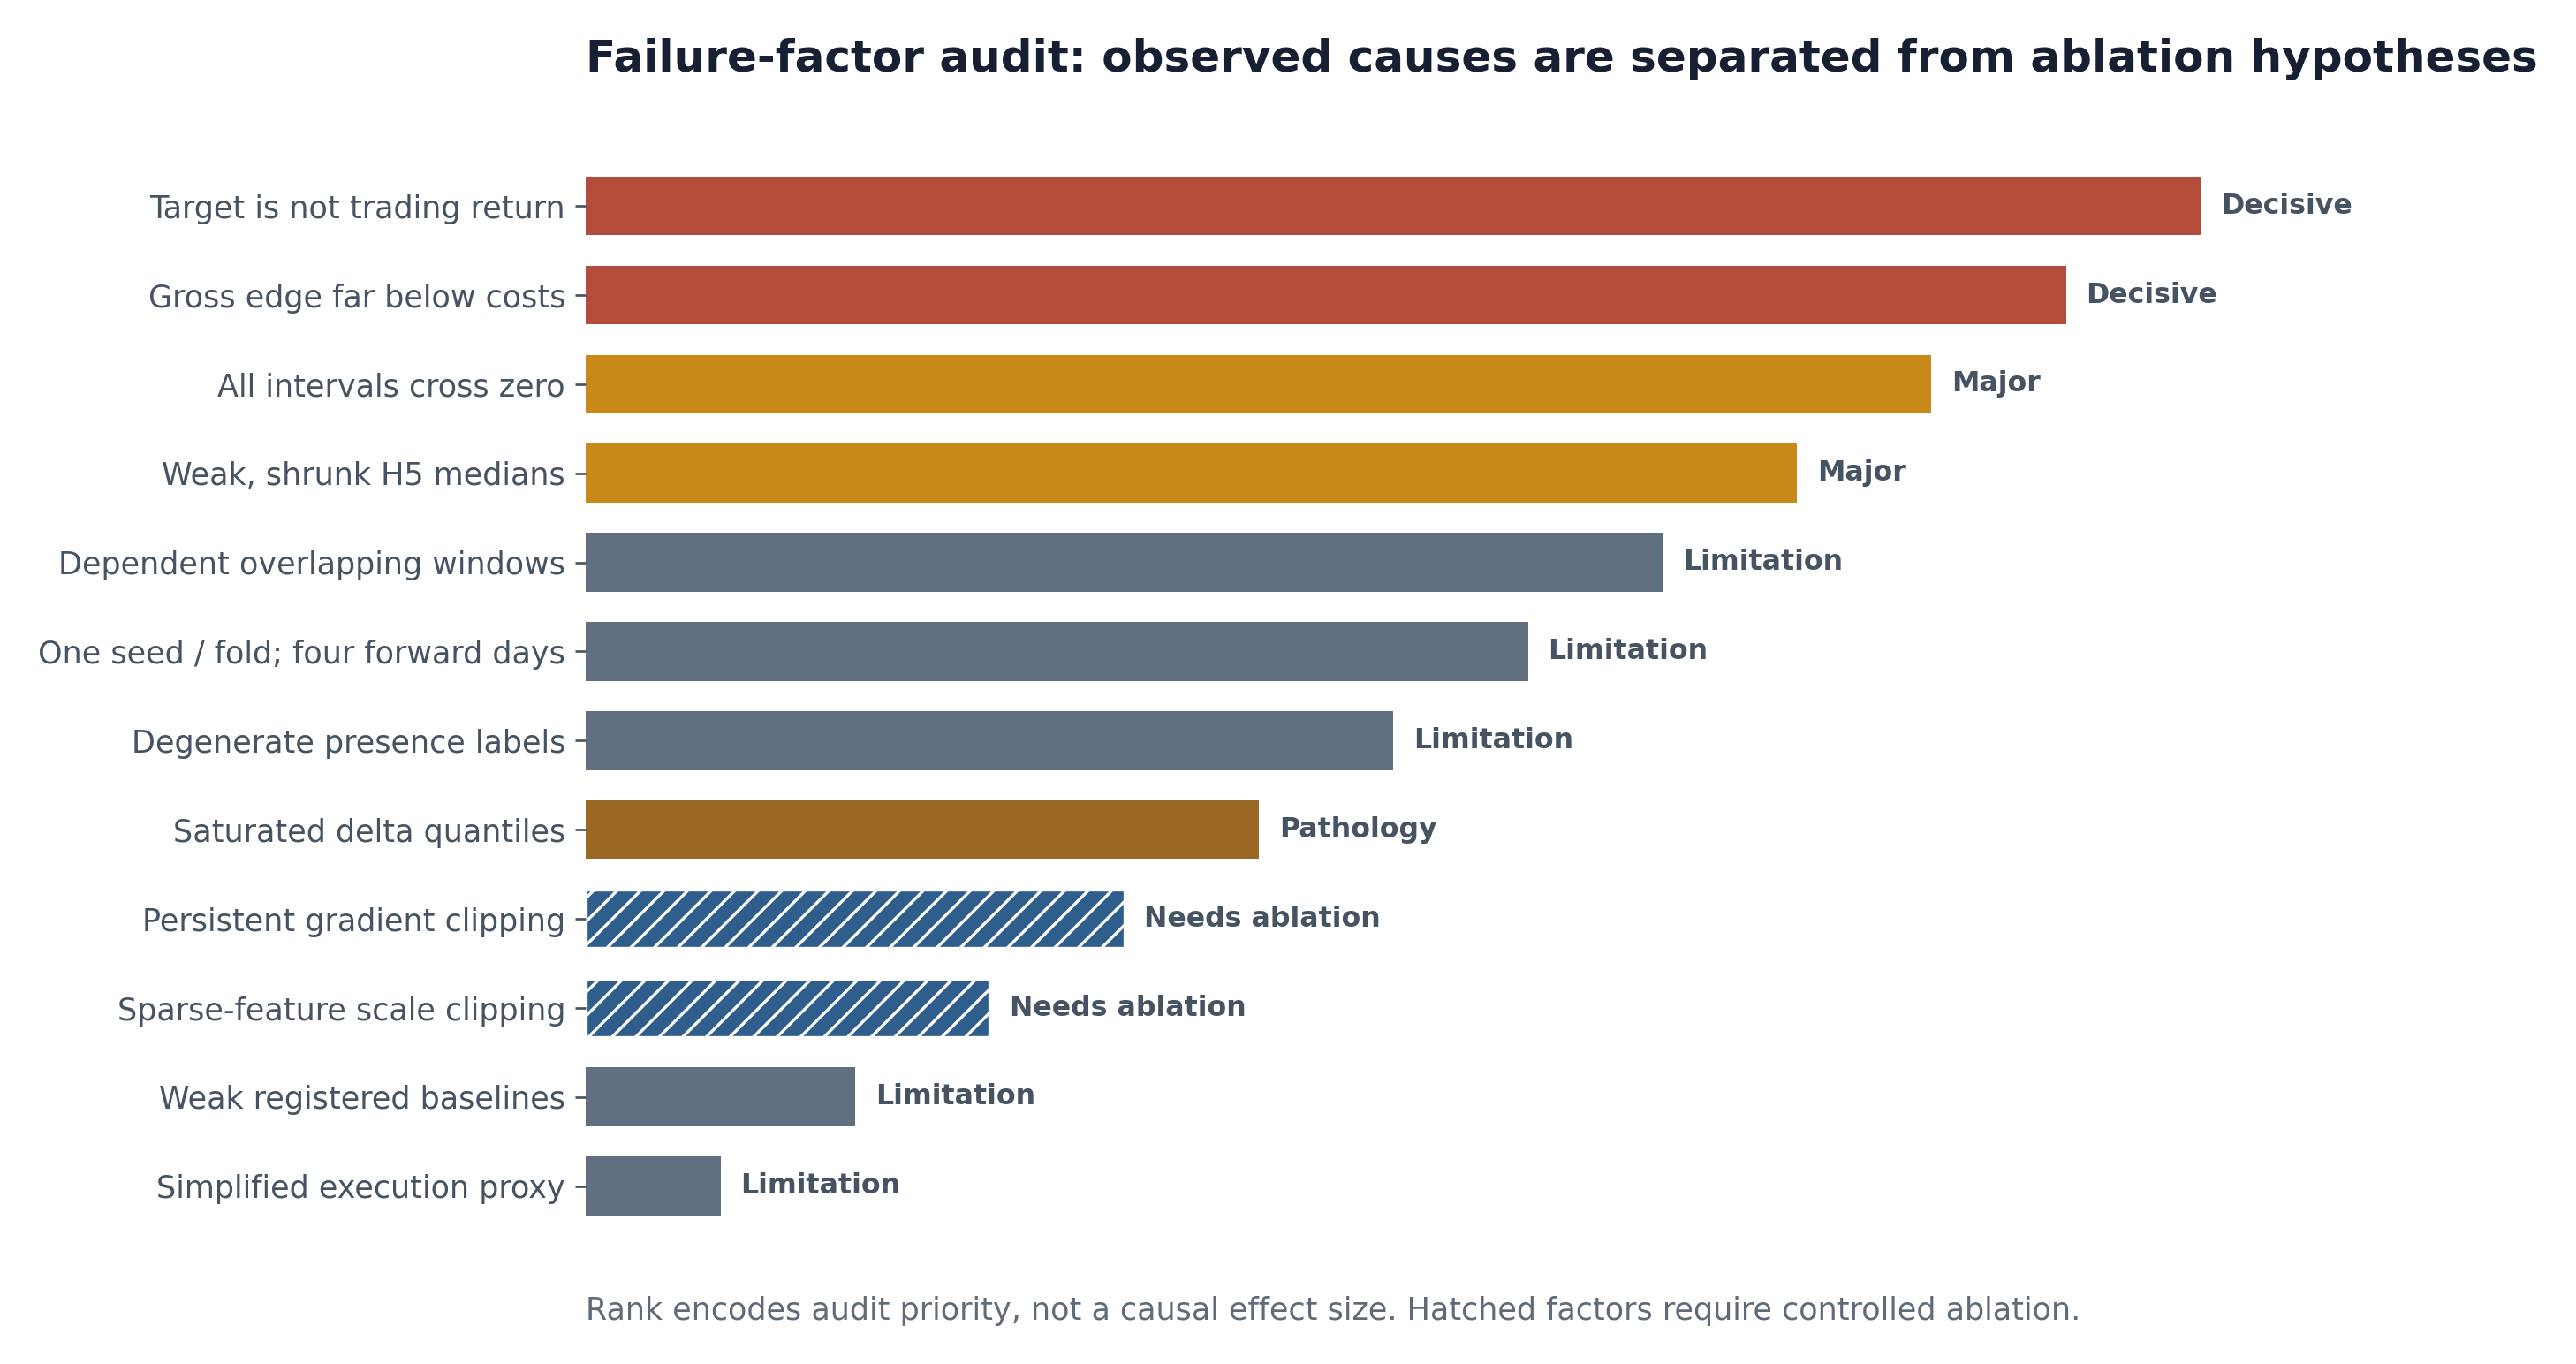
\includegraphics[width=0.91\textwidth]{assets/failure_map.png}
\caption{Ranked failure factors. Observed decisive and major factors are
separated from plausible contributors requiring prospective ablation.}
\label{fig:failure-map}
\end{figure}

\subsection{Decisive factors}

\paragraph{Task-decision mismatch.}
The model optimized five footprint primitives, not executable return or action.
Equation~\eqref{eq:h5-share} shows that only 3.46\% of nominal
horizon-target weighting concerned H5 total POC. Lower aggregate loss can
therefore coexist with an unchanged economic proxy.

\paragraph{Cost dominance.}
The long-flat gross edge of 0.4453 bps per round trip is structurally
incompatible with a 24-bps base round trip. Threshold search can change the
selected sample but cannot retroactively turn the observed 53.89-times
cost-to-break-even ratio into confirmatory evidence.

\paragraph{Uncertainty without selectivity.}
Every H5 interval crossed zero. The registered rule correctly abstained.
Forcing a median-sign trade discards the uncertainty information that the model
was explicitly trained to produce.

\subsection{Data, validation, and benchmark limitations}

Adjacent examples share most feature and label support. Training comprises
25,758 dependent rows from 18 sessions. With 2.09 million parameters, this is
approximately 81 parameters per nominal row and 116,086 per training session.
One seed, one fold, two selection days, and four forward days cannot estimate
seed instability, regime robustness, venue transfer, or tail behavior. The
retired final period removes the planned confirmatory window.

The empirical marginal baseline tests conditional structure relative to a
stationary marginal distribution. It does not establish whether attention,
hierarchy, or 2.09 million parameters are warranted. Ridge, logistic,
boosted-tree, temporal-convolutional, DeepLOB-like, persistence, and seasonal
baselines are still required.

\subsection{Target and output pathologies}

The three POC targets were correlated at roughly 0.93--0.97 and together
received
\begin{equation}
\frac{3}{3+0.5+0.5}=75\%
\label{eq:poc-weight}
\end{equation}
of target weighting. Buy and sell presence were positive for all relevant
forward examples, making the auxiliary classifier nearly constant. For an
all-positive label, \(\operatorname{BCE}(\eta,1)=\log(1+e^{-\eta})\to0\) as
\(\eta\to\infty\), so the task offers no directional selectivity.

For delta, the realized median was -0.0345, while the predicted-median
distribution had median 0.6695 and bias 0.6881; Pearson association was
-0.0107. The derivative
\begin{equation}
\frac{d}{dx}\tanh x=1-\tanh^2x\longrightarrow0
\quad\text{as}\quad|\tanh x|\longrightarrow1
\label{eq:tanh-saturation}
\end{equation}
describes why tail resolution vanishes near the bounds, but does not establish
the causal effect of saturation on aggregate performance.

Sparse L1 changes also interacted poorly with robust scaling. When
\(\operatorname{MAD}=0\), Equation~\eqref{eq:robust-scale} gives
\(s=10^{-6}\), so a deviation of only \(8\times10^{-6}\) reaches the clipping
boundary. Approximately 22.84\% of selected mid/bid/ask changes were clipped.
Persistent gradient clipping and sparse-feature clipping are observed, but
their metric effects require controlled retraining.

\begin{table}[!htbp]
\centering
\scriptsize
\begin{tabularx}{\textwidth}{@{}rY p{2.8cm}Y@{}}
\toprule
\textbf{Rank} & \textbf{Factor} & \textbf{Evidence status} &
\textbf{Implication}\\
\midrule
1 & Target is not trading return & Decisive, observed & Forecast loss is not a
PnL objective.\\
2 & Gross edge is far below costs & Decisive, observed & Tested policies are
economically infeasible.\\
3 & Every interval crosses zero & Major, observed & Registered policy abstains.\\
4 & Weak, shrunk H5 medians & Major, observed & Aggregate score masks weak
location signal.\\
5 & Heavy window overlap & Design limitation & Nominal sample size misleads.\\
6 & One seed/fold; four forward days & Validation limitation & Robustness is
unknown.\\
7 & Degenerate presence labels & Wasted capacity & Auxiliary classification
adds no selectivity.\\
8 & Saturated delta tails & Output pathology & Bounded uncertainty is
uninformative.\\
9 & Persistent gradient clipping & Plausible contributor & Requires optimizer
ablation.\\
10 & Sparse-feature clipping & Representation loss & Requires scaler ablation.\\
11 & Weak baseline set & Benchmark limitation & Transformer necessity is
untested.\\
12 & Simplified execution & Fidelity limitation & Live performance is
unestablished.\\
\bottomrule
\end{tabularx}
\caption{Failure-factor hierarchy.}
\label{tab:failure-factors}
\end{table}

\section{Threats to Validity}

\subsection{Internal and statistical conclusion validity}

The checkpoint and baseline were frozen before the forward evaluation, but
diagnostic policies and several decompositions were developed after inspecting
results. They are labeled post hoc. A single run cannot separate architecture
effects from initialization. Rows and labels are dependent, and only four
calendar days contribute to the estimate. Row-wise confidence intervals would
be anti-conservative; four daily blocks do not support a stable tail
probability. No significance claim, Sharpe inference, or probability of
profitability is reported.

\subsection{Construct and external validity}

Footprint POC and volume are not executable returns. Minute open/close trade
prices are not guaranteed fills. Fixed-bps costs omit dynamic spread, latency,
queue priority, impact, and partial execution. The evidence covers one venue,
one instrument, one month, one seed, one fold, and four forward days. It does
not establish transfer across assets, derivatives, venues, volatility regimes,
fee tiers, or live infrastructure.

\subsection{Researcher degrees of freedom}

The study has one registered forecast endpoint and one registered interval
policy, but the audit examines many cells and diagnostics. These analyses
generate hypotheses; they do not upgrade the original result. Future work must
freeze targets, baselines, thresholds, costs, folds, seeds, and stopping rules
before accessing a new confirmatory period.

\section{Corrective Research Protocol}

\begin{figure}[!htbp]
\centering
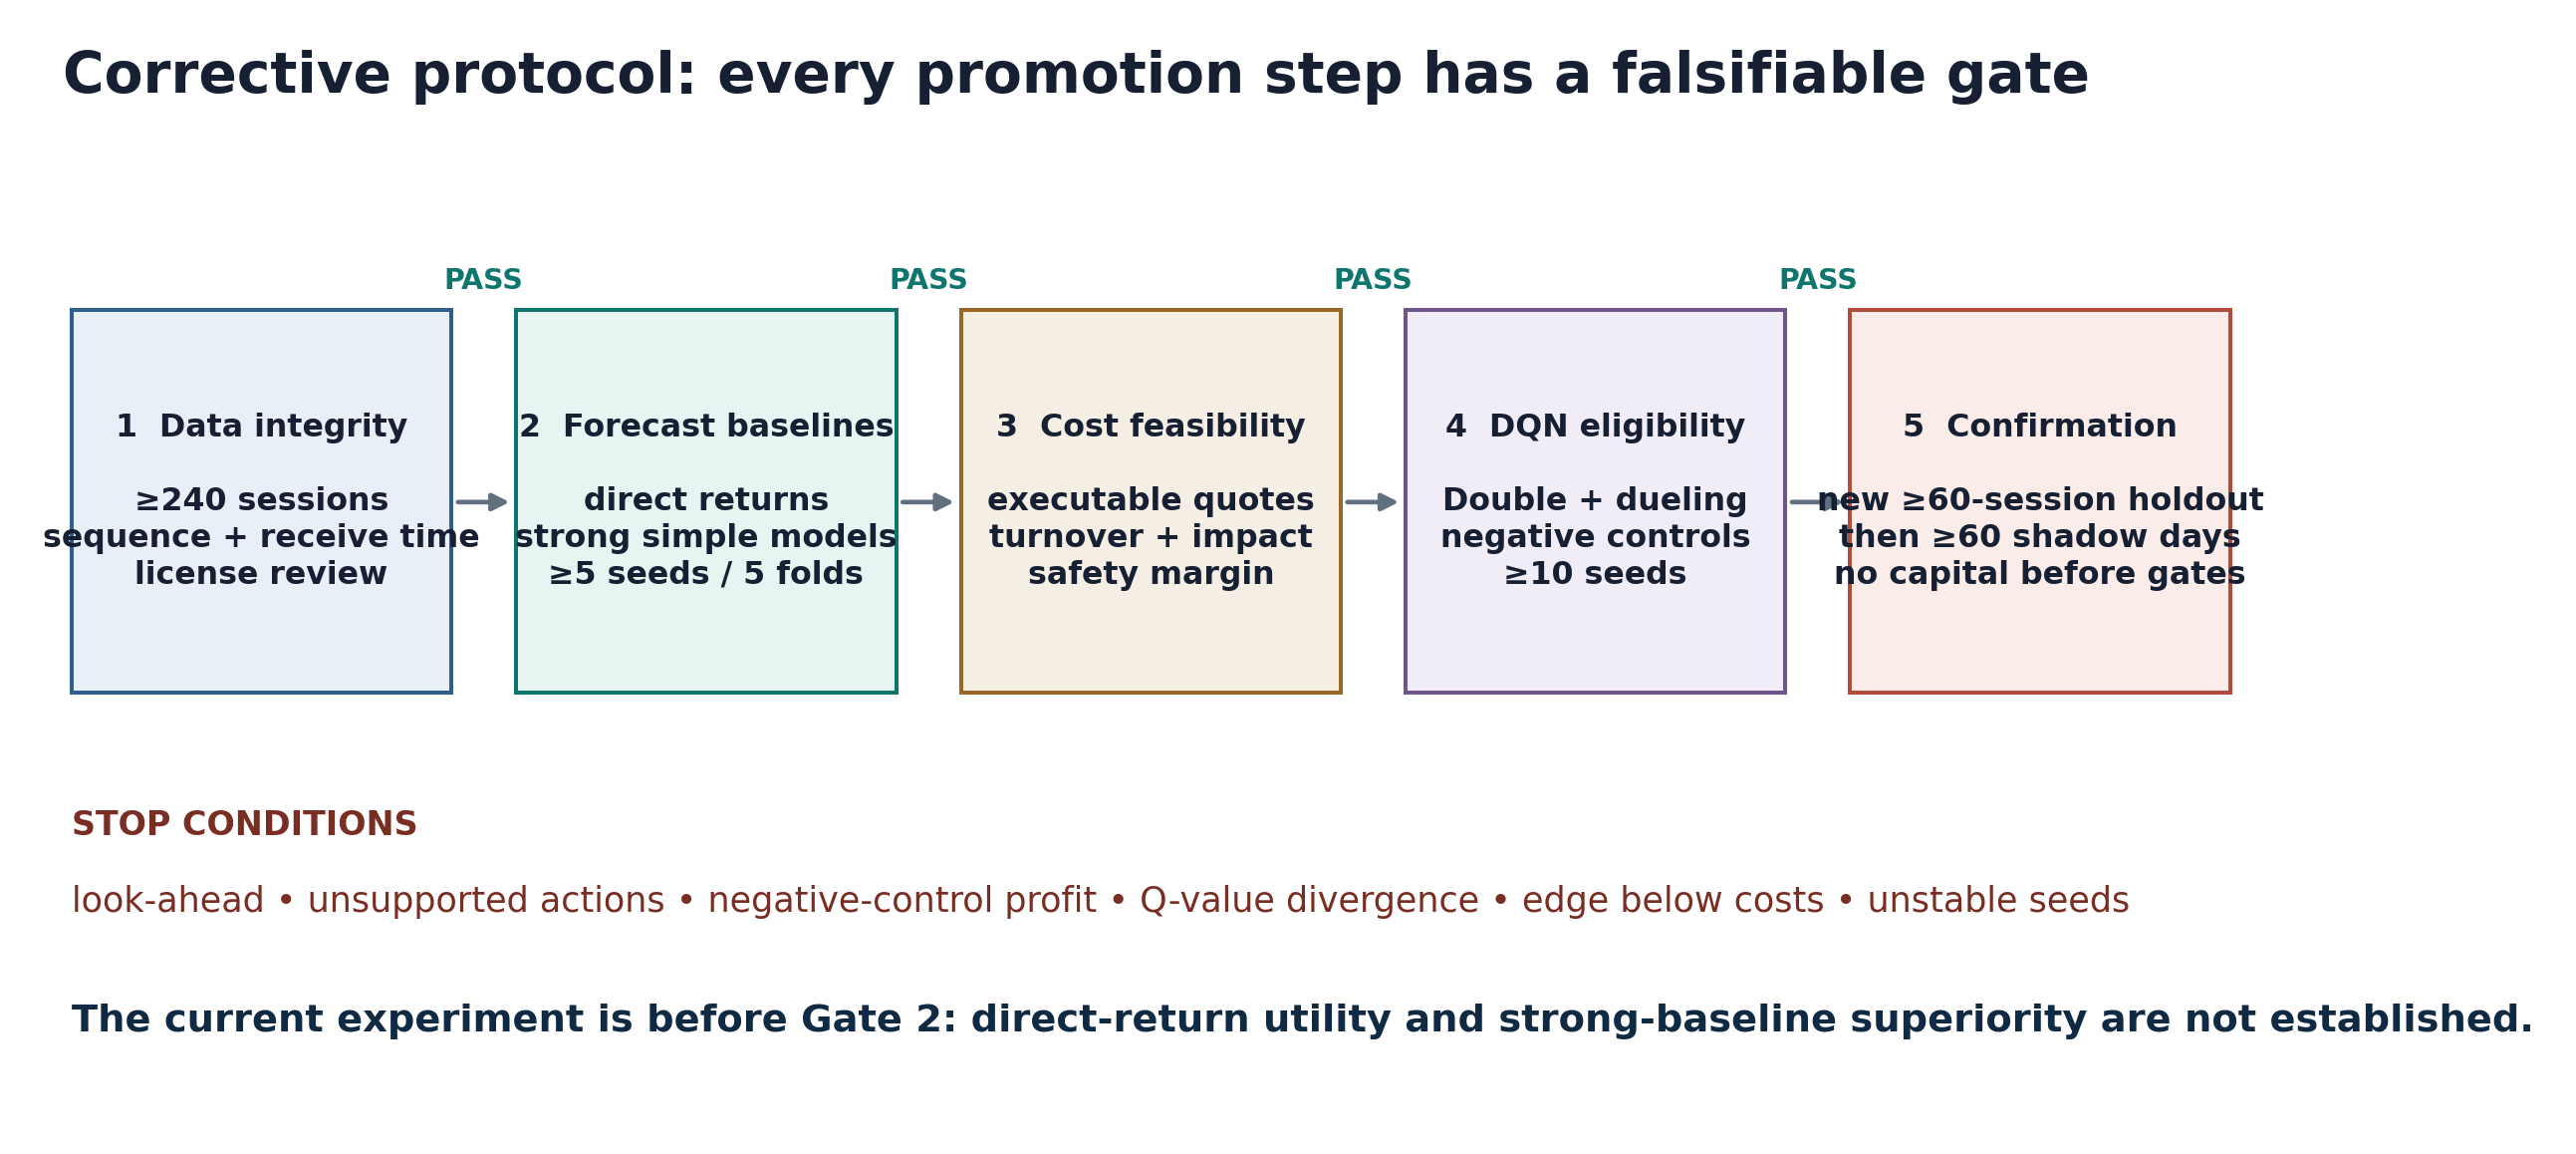
\includegraphics[width=0.94\textwidth]{assets/next_study.png}
\caption{Registered next-study gates. Forecast, execution, and reinforcement
learning require separate evidence and a newly sealed period.}
\label{fig:next-study}
\end{figure}

\subsection{Data and validation gates}

For cutoff \(c_i\), maximum lookback \(L_{\mathrm{lookback}}\), forecast span
\(H\Delta\), and label-completeness grace \(g_{\mathrm{label}}\), the full
dependency interval is
\begin{equation}
J_i=[c_i-L_{\mathrm{lookback}},
c_i+H\Delta+g_{\mathrm{label}}].
\label{eq:dependency-interval}
\end{equation}
Prospective train/test assignment must purge any observation whose \(J_i\)
crosses a fold boundary and apply an embargo at least as wide as the maximum
remaining dependency.

The next experiment should acquire at least 240 UTC sessions with exchange
event time and, where feasible, local receive time, sequence/checksum
integrity, historical instrument metadata, and a documented license review.
It should use at least five anchored rolling folds, each with at least 120
training, 20 selection, and 20 disjoint test sessions. At least five
Transformer seeds and ten finalist decision-model seeds are required. A new
access-controlled holdout of at least 60 sessions must remain target-inaccessible
until code, hashes, thresholds, costs, and endpoints are locked, followed by at
least 60 shadow-trading days before any capital decision.

\subsection{Targets, baselines, and economic gate}

Direct executable-return targets should be primary. Footprint targets should
remain only if incremental value survives ablation. Redundant POC heads should
be selected or orthogonalized; degenerate presence labels removed; and bounded
delta modeled with a distribution or transform compatible with its support.
Every complex candidate must be compared with frozen persistence/seasonal,
ridge/logistic, gradient-boosted, temporal-convolutional, and DeepLOB-like
baselines.

The primary endpoint should be net return under a preregistered execution model,
reported with turnover, drawdown, exposure, and capacity. The feasibility gate
is not positive frictionless return: a lower uncertainty bound for gross edge
must exceed estimated all-in cost by a frozen safety margin across folds and
seeds.

\section{Proposed Transformer--Double-DQN Study}

This section is a mathematical proposal only. No DQN has been implemented,
trained, backtested, or integrated, and no result in this paper comes from
reinforcement learning.

\subsection{State, action, transition, and reward}

The proposed state combines CHMT-Q embeddings, current target position,
realized volatility, spread/liquidity proxies, time-of-day, and risk-budget
variables. Actions specify next target position
\begin{equation}
a_t\in\{-1,0,+1\},
\label{eq:actions}
\end{equation}
rather than ambiguous buy/sell/hold events. With position \(p_t=a_t\), mid-price
change \(\Delta m_{t+1}\), transaction-cost function \(C_t\), and bounded risk
penalty \(\mathcal{R}_t\), shaped training reward would be
\begin{equation}
r_t=p_t\Delta m_{t+1}
-C_t(|p_t-p_{t-1}|,\mathrm{spread}_t,\mathrm{liquidity}_t)
-\lambda_{\mathrm{risk}}\mathcal{R}_t.
\label{eq:rl-reward}
\end{equation}
The reported endpoint must remain raw net PnL under the frozen simulator;
shaping is not business value. Historical transitions are valid only under the
explicit small-notional assumption that candidate actions do not alter future
market observations.

\subsection{Double-DQN and dueling derivation}

For discount \(\gamma\), online parameters \(\theta\), and target parameters
\(\bar\theta\), Double DQN separates action selection from evaluation:
\begin{align}
a_{t+1}^{*}&=\arg\max_{a'}Q_\theta(s_{t+1},a'),\nonumber\\
y_t^{\mathrm{DDQN}}&=r_t+\gamma(1-d_t)
Q_{\bar\theta}(s_{t+1},a_{t+1}^{*}),\nonumber\\
\mathcal{L}_{\mathrm{TD}}(\theta)
&=\E_{\mathcal{B}}\!\left[
H_\delta\!\left(Q_\theta(s_t,a_t)-y_t^{\mathrm{DDQN}}\right)
\right],
\label{eq:double-dqn}
\end{align}
where \(d_t\) marks termination and \(\mathcal{B}\) is replay data. The target
network would be updated slowly or periodically, with cadence frozen before
evaluation.

A dueling head decomposes
\begin{equation}
Q_\theta(s,a)=V_\theta(s)+A_\theta(s,a)
-\frac{1}{|\mathcal{A}|}\sum_{a'}A_\theta(s,a'),
\label{eq:dueling}
\end{equation}
where mean-centering identifies value and advantage. For offline data, a
conservative penalty may be ablated:
\begin{equation}
\mathcal{L}_{\mathrm{CQL}}
=\alpha\,
\E_s\!\left[
\log\sum_a e^{Q_\theta(s,a)}
-\E_{a\sim\mathcal{D}(\cdot\mid s)}Q_\theta(s,a)
\right].
\label{eq:cql}
\end{equation}
This discourages unsupported actions from receiving arbitrarily high values;
it does not validate the simulator or create action support.

\subsection{Eligibility and stopping gates}

\begin{table}[!htbp]
\centering
\small
\begin{tabularx}{\textwidth}{@{}Y Y Y@{}}
\toprule
\textbf{Gate} & \textbf{Minimum condition} & \textbf{Failure consequence}\\
\midrule
Data integrity & Sequence/receive-time and no-lookahead tests pass & Stop\\
Forecast utility & Direct-return model beats frozen simple baselines across
folds & Do not train DQN\\
Cost feasibility & Gross edge clears all-in costs with safety margin & Do not
train DQN\\
Offline support & Candidate actions have adequate state support & Restrict
actions or stop\\
Robustness & At least 5 encoder and 10 finalist DQN seeds & No promotion\\
Confirmation & New, sealed, at least 60-session holdout & No performance claim\\
Operations & At least 60 live shadow days & No capital allocation\\
\bottomrule
\end{tabularx}
\caption{Prerequisites for any future DQN study.}
\label{tab:dqn-gates}
\end{table}

Required controls include behavior cloning, no-change policies, randomized
rewards, shifted features, and permuted action labels. Profitable negative
controls indicate leakage or simulator error. Training must stop if action
support is inadequate, Q-values diverge, controls profit, or seed dispersion
exceeds a preregistered tolerance. Discount, target-update cadence, replay
sampling, and multi-step return length remain unspecified and must be frozen
before implementation.

\section{Reproducibility, Availability, and Ethics}

\subsection{Artifact ledger}

\begin{longtable}{@{}p{3.1cm}p{9.4cm}p{2.2cm}@{}}
\caption{Immutable local artifact ledger.}\label{tab:artifacts}\\
\toprule
\textbf{Artifact} & \textbf{SHA-256 or identifier} & \textbf{Role}\\
\midrule
\endfirsthead
\toprule
\textbf{Artifact} & \textbf{SHA-256 or identifier} & \textbf{Role}\\
\midrule
\endhead
Compiled dataset &
\nolinkurl{565c1d8e912ee426a1a92572d5be481ec5168d54d1ae53bd77fdd70d888e4df6}
& Dataset identity\\
Dataset manifest &
\nolinkurl{68ec9eca21d2a30546435738e8e07d565a64edbf01825246db659a4c1bb98046}
& Source/shard manifest\\
Compiler report &
\nolinkurl{cc3f9208e2410b41ca9836ef762c15cfd91d3b9c704c2d198c438425f4c9e8ba}
& Compilation audit\\
Dependency lock &
\nolinkurl{48792cf2789a576553fc29b1b727e97342d28fed1fdbeb91c31135a84bfff898}
& Environment identity\\
Source split &
\nolinkurl{7f5254f62a3d70a6f02e41b1991f25d3bd8338e7aa9b25c5fa19737f70a7bb8e}
& Partition identity\\
Input/target scaler &
\nolinkurl{29a733fac9986eb7e879555b6813f8d35b06c98dee9041057e6fc4287bd50880}
& Scaling state\\
Training run &
\nolinkurl{25be2f446a75ad37120bba956ea86e46c0ecefa004ab3343d6745cdbee102fb3}
& Experiment identity\\
Study protocol &
\nolinkurl{885fcd0fee23115a4a5480ec94d95f436e251ec0caf796f9686867ed7e72f5d0}
& Frozen protocol\\
Prediction tape &
\nolinkurl{27d9ffbe41b18868b8a45bf9c48c936908de7394dd6ecfec7062cc531cc7e1f0}
& Model outputs\\
Study results &
\nolinkurl{083da170146585cf1a16dde56e2da02697194640ed7b053d3298d8e3775bee6a}
& Results ledger\\
Failure diagnostics &
\nolinkurl{ece5b18f8a8455f7edac8491b6d23362fa14f618129b1193b1febf14bc89505e}
& Audit results\\
DQN plan &
\nolinkurl{d5e81f203619c55754c940df7e92ec5995e4db41b3a7d6f3db4137318f7a502c}
& Future-work specification\\
\bottomrule
\end{longtable}

The implementation and local artifacts are private research materials. Raw
exchange archives, derived Arrow data, the prediction tape, weights, and
checkpoints are not redistributed. Reproduction requires independent data
acquisition under applicable OKX terms and regeneration under the disclosed
tensor, split, training, and evaluation contracts. Hashes establish local
identity; they do not substitute for public data availability.

\subsection{Risk and declarations}

The model is unsuitable for capital allocation. Any later live test requires
shadow mode, hard position/loss limits, kill switches, human oversight, and
monitoring for drift, latency, execution quality, and turnover.

\begin{description}[leftmargin=3.6cm,style=nextline]
\item[Funding] To be completed by the authors.
\item[Competing interests] To be completed by the authors.
\item[Author contributions] To be completed using the selected venue taxonomy.
\item[Generative tools] To be declared according to venue policy. Human authors
must independently verify every claim, equation, reference, table, and figure.
\item[Data and code] Private local research artifacts; no redistribution claim.
\item[Human or animal participants] Not applicable.
\end{description}

\section{Conclusion}

CHMT-Q improved a registered aggregate proper score by 2.26\% on a four-session
development-forward partition. That result did not imply a useful trading
signal. H5 medians were weak and under-dispersed, every uncertainty interval
crossed zero, the registered policy made no trades, and diagnostic policies
lost heavily once fixed costs were applied. The observed long-flat gross edge
was 53.89 times too small for the base cost assumption.

The strongest contribution is methodological. Proper scores, conditional
signal, and executable economics are distinct evidentiary levels. A model
should not advance because it wins at the first while failing or remaining
untested at the others. The current checkpoint remains research-only and
non-promotable. A larger, access-controlled, multi-fold, multi-seed study with
direct return targets, strong baselines, realistic execution, and a new sealed
holdout is required before reconsideration. The proposed
Transformer--Double-DQN design is one testable option inside that protocol, not
a remedy already demonstrated.

\appendix

\section{Detailed Derivations and Checks}

\subsection{Ordered-head proof after bounded transformation}

\begin{lemma}
Let \(q_L=c-\softplus(a)\), \(q_M=c\), \(q_U=c+\softplus(b)\). If
\(f:\R\rightarrow\R\) is nondecreasing, then
\(f(q_L)\leq f(q_M)\leq f(q_U)\).
\end{lemma}
\begin{proof}
\(\softplus(a),\softplus(b)>0\) implies \(q_L<q_M<q_U\). The definition of a
nondecreasing function preserves both inequalities. Taking \(f=\tanh\) proves
ordered bounded delta quantiles. Strict mathematical order may become numerical
equality in saturated floating-point tails.
\end{proof}

\subsection{Aggregate score decomposition}

Let \(N_{hk}\) denote the weighted sum of pinball losses for cell \((h,k)\) and
\(D_{hk}\) its mask/weight denominator. Then
\begin{equation}
\mathcal{L}_Q
=\frac{\sum_{h,k}N_{hk}}{\sum_{h,k}D_{hk}}
=\sum_{h,k}\omega_{hk}\mathcal{L}_{hk},\qquad
\omega_{hk}=\frac{D_{hk}}{\sum_{h',k'}D_{h'k'}}.
\label{eq:score-decomposition}
\end{equation}
An aggregate improvement therefore permits negative cell improvements whenever
positive, high-weight cells dominate. In this run, the three correlated POC
targets carry most target weight, while log-volume and delta deterioration is
downweighted.

\subsection{Proper-score and trading-value counterexample}

Consider \(X\sim\mathcal{N}(0,1)\),
\(Y=X+\epsilon\) with \(\epsilon\sim\mathcal{N}(0,\sigma^2)\), and executable
return \(R=\eta\) with \(\eta\) independent and symmetric. The conditional
median forecast \(q_{0.5}(X)=X\) strictly improves expected absolute/pinball
loss over the unconditional median 0 whenever \(X\) is nondegenerate. Yet
\(\E[R\mid X,Y]=0\), so for any position \(a\),
\begin{equation}
\E[aR-C|a|\mid X,Y]=-C|a|\leq0,
\label{eq:counterexample}
\end{equation}
with strict loss for \(a\neq0\) and \(C>0\). This formalizes why score
improvement cannot, without a target-decision bridge, establish edge.

\subsection{Cost compounding}

For constant small gross arithmetic edge \(g\) and round-trip cost \(2c\) over
\(N\) trades,
\begin{equation}
R_N=(1+g-2c)^N-1.
\label{eq:cost-compounding}
\end{equation}
The first-order log approximation is
\begin{equation}
\log(1+R_N)
=N\log(1+g-2c)\approx N(g-2c)
-\frac{N}{2}(g-2c)^2.
\label{eq:log-cost}
\end{equation}
Even a positive frictionless \(g\) compounds rapidly downward when \(2c>g\).
This explains the large negative cost-adjusted returns without invoking
leverage.

\subsection{Parameter ledger reconciliation}

For a biased linear map \(a\rightarrow b\),
\begin{equation}
P_{\mathrm{linear}}(a,b)=ab+b,
\label{eq:linear-params}
\end{equation}
and a biased SwiGLU block \(d\rightarrow f\rightarrow d\) has
\begin{equation}
P_{\mathrm{SwiGLU}}(d,f)=3df+2f+d.
\label{eq:swiglu-params}
\end{equation}
Together with attention projections, normalizers, LayerScale vectors,
embeddings, gates, and learned head temperatures, the component ledger is:

\begin{table}[H]
\centering
\small
\begin{tabular}{@{}lr@{}}
\toprule
\textbf{Component} & \textbf{Trainable parameters}\\
\midrule
Bar, L1, and level projections & 4,768\\
Quality MLP & 18,688\\
Bar time MLP & 4,768\\
L1 patch-time MLP & 4,832\\
L2 patch-time MLP & 4,832\\
Modality embeddings & 384\\
L2 side/rank embeddings & 384\\
L2 level CHMT block & 10,660\\
Book query, norm, and 32-to-128 projection & 4,288\\
L1/L2 patch embeddings and pool MLPs & 9,346\\
Nine temporal CHMT blocks & 1,489,608\\
Two decoder blocks & 463,632\\
Three modality gate MLPs & 49,539\\
Fusion norm and context projection & 16,640\\
Horizon queries and horizon MLP & 4,992\\
Shared 128-to-17 head & 2,193\\
\midrule
\textbf{Total} & \textbf{2,089,554}\\
\bottomrule
\end{tabular}
\caption{Exact implemented parameter ledger. The total includes 36 learned
per-head Q/K temperatures omitted from the superseded 2,089,518 arithmetic.}
\label{tab:parameters}
\end{table}

\section{Notation}

\begin{longtable}{@{}p{2.8cm}p{11.2cm}@{}}
\caption{Principal notation.}\label{tab:notation}\\
\toprule
\textbf{Symbol} & \textbf{Meaning}\\
\midrule
\endfirsthead
\toprule
\textbf{Symbol} & \textbf{Meaning}\\
\midrule
\endhead
\(B\) & Batch size\\
\(c\) & Forecast decision cutoff\\
\(\mathcal{F}_c\) & Information available by cutoff\\
\(H\) & Number of direct forecast horizons, five\\
\(p_{\mathrm{ref}}\) & Causal reference price\\
\(\delta_p\) & Instrument tick size\\
\(\ell_{\mathrm{ref}}\) & Causal trailing log-volume reference\\
\(d,d_h,d_{\mathrm{ff}}\) & Model, attention-head, and feed-forward widths\\
\(m\) & Boolean validity/eligibility mask\\
\(\alpha_m\) & Normalized modality gate\\
\(Q_\tau\) & Conditional quantile at level \(\tau\)\\
\(\rho_\tau\) & Pinball loss\\
\(\theta\) & Learned model parameters\\
\(p_t\) & Target trading position\\
\(\kappa_{\mathrm{BE}}\) & Break-even one-way transaction cost\\
\bottomrule
\end{longtable}

\section{Registered and Post Hoc Analyses}

\begin{table}[H]
\centering
\small
\begin{tabularx}{\textwidth}{@{}Y p{3.8cm}Y@{}}
\toprule
\textbf{Analysis} & \textbf{Status} & \textbf{Interpretation}\\
\midrule
Weighted normalized pinball versus empirical marginal &
Registered forecast endpoint & Development evidence\\
Interval long-flat policy at base costs &
Registered economic endpoint & Zero trades; development evidence\\
Median-sign long-flat and long-short policies &
Diagnostic post hoc & Cost-feasibility diagnosis only\\
Anchor-close candle direction proxy &
Diagnostic post hoc & Approximate downstream association\\
Per-target/per-horizon heatmaps &
Diagnostic decomposition & Explains aggregate heterogeneity\\
Recent-three-day and hour baselines &
Post hoc; not in primary comparison & Hypothesis generation only\\
DQN architecture and validation plan &
Proposed future work & No performance evidence\\
\bottomrule
\end{tabularx}
\caption{Status of analyses.}
\label{tab:analysis-status}
\end{table}

\section{Submission Completion Items}

\begin{enumerate}
  \item Complete affiliation, correspondence, ORCID, funding,
  competing-interest, contribution, and tool-use fields as required.
  \item Select the target venue and apply its exact class and bibliography
  requirements without altering the empirical claims.
  \item Independently recompute and verify every quantitative table and figure
  from immutable artifacts.
  \item Preserve the holdout-integrity disclosure; never relabel June 25--30 as
  sealed, untouched, or confirmatory.
  \item Confirm that the venue permits private code/data with a regeneration
  contract, or choose an appropriate controlled archive and release policy.
\end{enumerate}

\small
\begin{thebibliography}{30}

\bibitem{vaswani2017}
A.~Vaswani et al.
\newblock Attention is all you need.
\newblock \emph{Advances in Neural Information Processing Systems}, 30, 2017.
\newblock \url{https://arxiv.org/abs/1706.03762}.

\bibitem{shaw2018}
P.~Shaw, J.~Uszkoreit, and A.~Vaswani.
\newblock Self-attention with relative position representations.
\newblock \emph{NAACL-HLT}, pages 464--468, 2018.
\newblock \url{https://doi.org/10.18653/v1/N18-2074}.

\bibitem{zhang2019rms}
B.~Zhang and R.~Sennrich.
\newblock Root mean square layer normalization.
\newblock \emph{Advances in Neural Information Processing Systems}, 32, 2019.
\newblock \url{https://arxiv.org/abs/1910.07467}.

\bibitem{shazeer2020}
N.~Shazeer.
\newblock GLU variants improve Transformer.
\newblock Technical report, 2020.
\newblock \url{https://arxiv.org/abs/2002.05202}.

\bibitem{nie2023}
Y.~Nie et al.
\newblock A time series is worth 64 words: Long-term forecasting with
Transformers.
\newblock \emph{International Conference on Learning Representations}, 2023.
\newblock \url{https://arxiv.org/abs/2211.14730}.

\bibitem{liu2024}
Y.~Liu et al.
\newblock iTransformer: Inverted Transformers are effective for time series
forecasting.
\newblock \emph{International Conference on Learning Representations}, 2024.
\newblock \url{https://arxiv.org/abs/2310.06625}.

\bibitem{lim2021}
B.~Lim, S.~O. Arik, N.~Loeff, and T.~Pfister.
\newblock Temporal fusion Transformers for interpretable multi-horizon time
series forecasting.
\newblock \emph{International Journal of Forecasting}, 37(4):1748--1764, 2021.
\newblock \url{https://doi.org/10.1016/j.ijforecast.2021.03.012}.

\bibitem{zeng2023}
A.~Zeng et al.
\newblock Are Transformers effective for time series forecasting?
\newblock \emph{AAAI}, 37(9):11121--11128, 2023.
\newblock \url{https://doi.org/10.1609/aaai.v37i9.26317}.

\bibitem{deepLOB2019}
Z.~Zhang, S.~Zohren, and S.~Roberts.
\newblock DeepLOB: Deep convolutional neural networks for limit order books.
\newblock \emph{IEEE Transactions on Signal Processing}, 67(11):3001--3012,
2019.
\newblock \url{https://doi.org/10.1109/TSP.2019.2907260}.

\bibitem{wallbridge2020}
J.~Wallbridge.
\newblock Transformers for limit order books.
\newblock Technical report, 2020.
\newblock \url{https://arxiv.org/abs/2003.00130}.

\bibitem{zhang2021lob}
Z.~Zhang and S.~Zohren.
\newblock Multi-horizon forecasting for limit order books: Novel deep learning
approaches and hardware acceleration using intelligent processing units.
\newblock Technical report, 2021.
\newblock \url{https://arxiv.org/abs/2105.10430}.

\bibitem{ntakaris2018}
A.~Ntakaris et al.
\newblock Benchmark dataset for mid-price forecasting of limit order book data
with machine learning methods.
\newblock \emph{Journal of Forecasting}, 37(8):852--866, 2018.
\newblock \url{https://doi.org/10.1002/for.2543}.

\bibitem{kolm2023}
P.~N. Kolm, J.~Turiel, and N.~Westray.
\newblock Deep order flow imbalance: Extracting alpha at multiple horizons from
the limit order book.
\newblock \emph{Mathematical Finance}, 33(4):1044--1081, 2023.
\newblock \url{https://doi.org/10.1111/mafi.12413}.

\bibitem{lucchese2024}
L.~Lucchese, M.~S. Pakkanen, and A.~E.~D. Veraart.
\newblock The short-term predictability of returns in order book markets: A
deep learning perspective.
\newblock \emph{International Journal of Forecasting}, 40(4):1607--1626, 2024.
\newblock \url{https://doi.org/10.1016/j.ijforecast.2024.02.001}.

\bibitem{briola2025}
A.~Briola, S.~Bartolucci, and T.~Aste.
\newblock Deep limit order book forecasting: A microstructural guide.
\newblock \emph{Quantitative Finance}, 2025.
\newblock \url{https://doi.org/10.1080/14697688.2025.2522911}.

\bibitem{gneiting2007}
T.~Gneiting and A.~E. Raftery.
\newblock Strictly proper scoring rules, prediction, and estimation.
\newblock \emph{Journal of the American Statistical Association},
102(477):359--378, 2007.
\newblock \url{https://doi.org/10.1198/016214506000001437}.

\bibitem{romano2019}
Y.~Romano, E.~Patterson, and E.~J. Candes.
\newblock Conformalized quantile regression.
\newblock \emph{Advances in Neural Information Processing Systems}, 32, 2019.
\newblock \url{https://arxiv.org/abs/1905.03222}.

\bibitem{sirignano2019}
J.~Sirignano and R.~Cont.
\newblock Universal features of price formation in financial markets:
Perspectives from deep learning.
\newblock \emph{Quantitative Finance}, 19(9):1449--1459, 2019.
\newblock \url{https://doi.org/10.1080/14697688.2019.1622295}.

\bibitem{white2000}
H.~White.
\newblock A reality check for data snooping.
\newblock \emph{Econometrica}, 68(5):1097--1126, 2000.
\newblock \url{https://doi.org/10.1111/1468-0262.00152}.

\bibitem{politis1994}
D.~N. Politis and J.~P. Romano.
\newblock The stationary bootstrap.
\newblock \emph{Journal of the American Statistical Association},
89(428):1303--1313, 1994.
\newblock \url{https://doi.org/10.1080/01621459.1994.10476870}.

\bibitem{harvey2016}
C.~R. Harvey, Y.~Liu, and H.~Zhu.
\newblock \ldots and the cross-section of expected returns.
\newblock \emph{Review of Financial Studies}, 29(1):5--68, 2016.
\newblock \url{https://doi.org/10.1093/rfs/hhv059}.

\bibitem{mnih2015}
V.~Mnih et al.
\newblock Human-level control through deep reinforcement learning.
\newblock \emph{Nature}, 518:529--533, 2015.
\newblock \url{https://doi.org/10.1038/nature14236}.

\bibitem{hasselt2016}
H.~van Hasselt, A.~Guez, and D.~Silver.
\newblock Deep reinforcement learning with Double Q-learning.
\newblock \emph{AAAI}, 30(1):2094--2100, 2016.
\newblock \url{https://doi.org/10.1609/aaai.v30i1.10295}.

\bibitem{wang2016dueling}
Z.~Wang, T.~Schaul, M.~Hessel, H.~van Hasselt, M.~Lanctot, and N.~de Freitas.
\newblock Dueling network architectures for deep reinforcement learning.
\newblock \emph{Proceedings of Machine Learning Research}, 48:1995--2003, 2016.
\newblock \url{https://proceedings.mlr.press/v48/wangf16.html}.

\bibitem{dabney2018}
W.~Dabney, M.~Rowland, M.~Bellemare, and R.~Munos.
\newblock Distributional reinforcement learning with quantile regression.
\newblock \emph{AAAI}, 32(1), 2018.
\newblock \url{https://doi.org/10.1609/aaai.v32i1.11791}.

\bibitem{kumar2020}
A.~Kumar, A.~Zhou, G.~Tucker, and S.~Levine.
\newblock Conservative Q-learning for offline reinforcement learning.
\newblock \emph{Advances in Neural Information Processing Systems},
33:1179--1191, 2020.
\newblock \url{https://arxiv.org/abs/2006.04779}.

\bibitem{levine2020}
S.~Levine, A.~Kumar, G.~Tucker, and J.~Fu.
\newblock Offline reinforcement learning: Tutorial, review, and perspectives on
open problems.
\newblock Technical report, 2020.
\newblock \url{https://arxiv.org/abs/2005.01643}.

\bibitem{henderson2018}
P.~Henderson et al.
\newblock Deep reinforcement learning that matters.
\newblock \emph{AAAI}, 32(1), 2018.
\newblock \url{https://doi.org/10.1609/aaai.v32i1.11694}.

\bibitem{bailey2017}
D.~H. Bailey, J.~M. Borwein, M.~Lopez de Prado, and Q.~J. Zhu.
\newblock The probability of backtest overfitting.
\newblock \emph{Journal of Computational Finance}, 20(4):39--69, 2017.
\newblock \url{https://doi.org/10.21314/JCF.2016.322}.

\bibitem{racine2000}
J.~Racine.
\newblock Consistent cross-validatory model-selection for dependent data:
hv-block cross-validation.
\newblock \emph{Journal of Econometrics}, 99(1):39--61, 2000.
\newblock \url{https://doi.org/10.1016/S0304-4076(00)00030-0}.

\end{thebibliography}

\end{document}
